% Created 2014-12-31 Wed 12:27
\documentclass[11pt]{article}
\usepackage[utf8]{inputenc}
\usepackage[T1]{fontenc}
\usepackage{fixltx2e}
\usepackage{graphicx}
\usepackage{longtable}
\usepackage{float}
\usepackage{wrapfig}
\usepackage{rotating}
\usepackage[normalem]{ulem}
\usepackage{amsmath}
\usepackage{textcomp}
\usepackage{marvosym}
\usepackage{wasysym}
\usepackage{amssymb}
\usepackage{hyperref}
\tolerance=1000
\date{\today}
\title{Bare Metal Provisioning with Oracle Enteprise Manager}
\hypersetup{
  pdfkeywords={},
  pdfsubject={},
  pdfcreator={Emacs 24.4.1 (Org mode 8.2.10)}}
\begin{document}

\maketitle
\tableofcontents

\section{Overview}
\label{sec-1}
\section{Conventions used in this document}
\label{sec-2}
Text to be typed in is shown in this face: \texttt{type me in}

GUI menu options will be shown connected by arrows, thus: Top -> Child1 -> Child2 -> Leaf.


\section{Current Environment}
\label{sec-3}
\section{Setup}
\label{sec-4}
The following steps need to be taken once, to allow the browser to access the Oracle Enterprise Manager (OEM) GUI, and to prepare the OEM environment for Bare Metal Provisioning (BMP).

Accessing OEM is through the OEM URL: \texttt{https://HOST:17802/em} where \texttt{HOST} is the (resolvable) hostname or ip address of the host machine. (It is assumed that the local firewall permits port 17802 to be accessed).
\subsection{Browser Certificates}
\label{sec-4-1}
Connect to the OEM URL. Your browser will likely show a security exception (the image below is shown using Firefox 31.2.0):
\begin{figure}[htb]
\centering
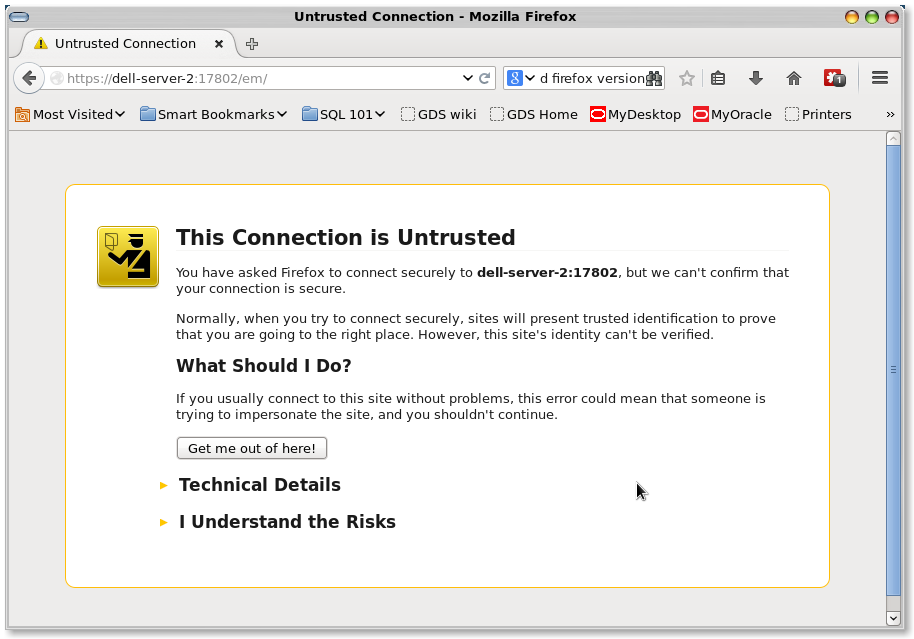
\includegraphics[width=.9\linewidth]{images/Browser_Certificate_1.png}
\caption{Initial Untrusted Certificate Screen}
\end{figure}
\clearpage
Click on the lower yellow triangle to expose the 'Add Exception\ldots{}' button:
\begin{figure}[htb]
\centering
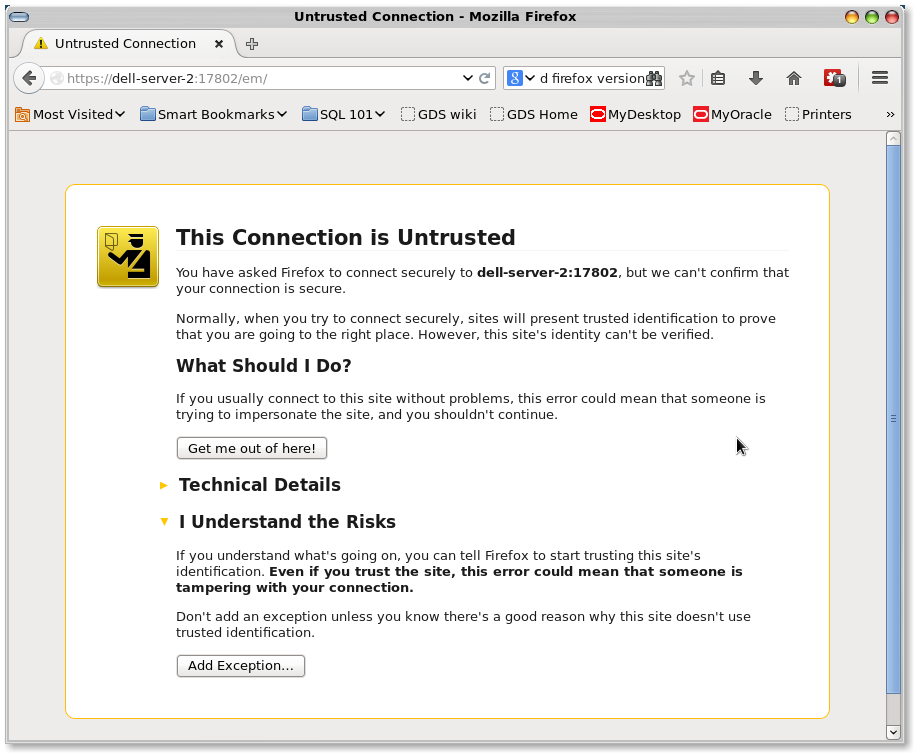
\includegraphics[width=.9\linewidth]{images/Browser_Certificate_2.png}
\caption{Untrusted Connection showing 'Add Exception\ldots{}' Button}
\end{figure}
\clearpage
Add the exception by clicking the 'Add Exception\ldots{}' button:
\begin{figure}[htb]
\centering
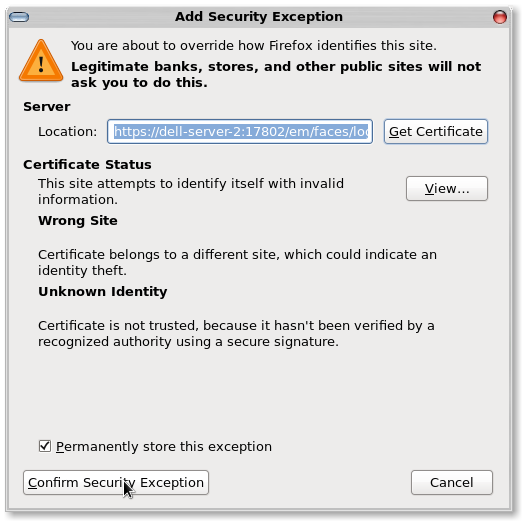
\includegraphics[width=.9\linewidth]{images/Browser_Certificate_3.png}
\caption{Add Security Exception}
\end{figure}
\clearpage
And then clicking the 'Confirm Security Exception' button. This will then take you to the OEM login window:
\begin{figure}[htb]
\centering
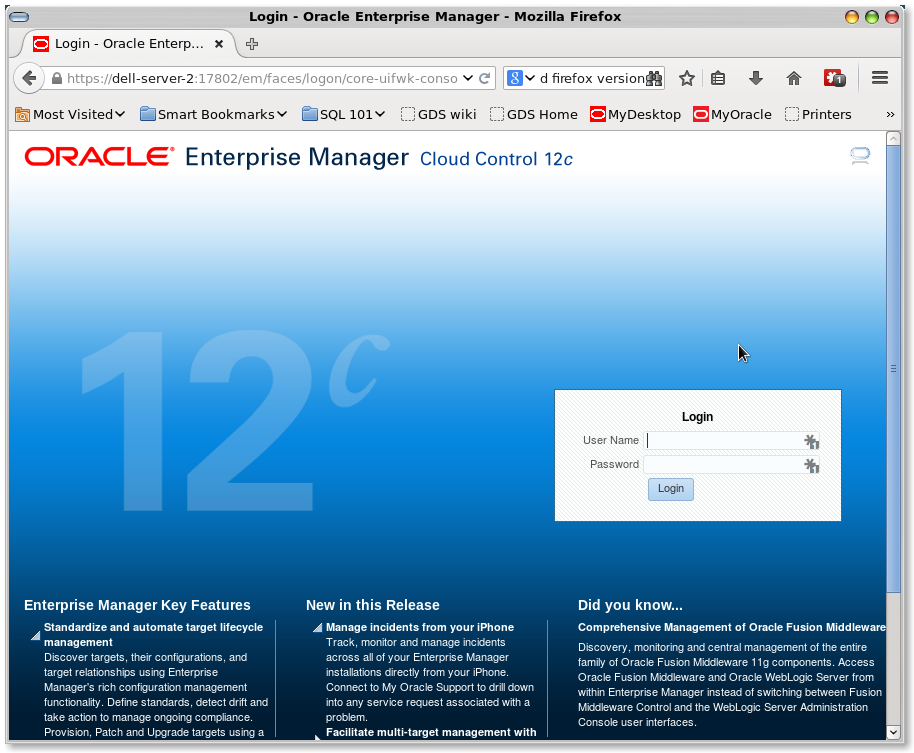
\includegraphics[width=.9\linewidth]{images/Screenshot-Login-OracleEnterpriseManager-MozillaFirefox.png}
\caption{OEM Login}
\end{figure}
\clearpage
\subsection{Oracle Enterprise Manager GUI setup}
\label{sec-4-2}
Login to OEM by accessing the OEM URL and using the name/password pair of 'sysman/Welcome1'. This will show you an 'Accessibility Preferences' page (this is \textbf{not} actually the page you'll first see! However the initial page is very similar, so hopefully this image is sufficient!):
\begin{figure}[htb]
\centering
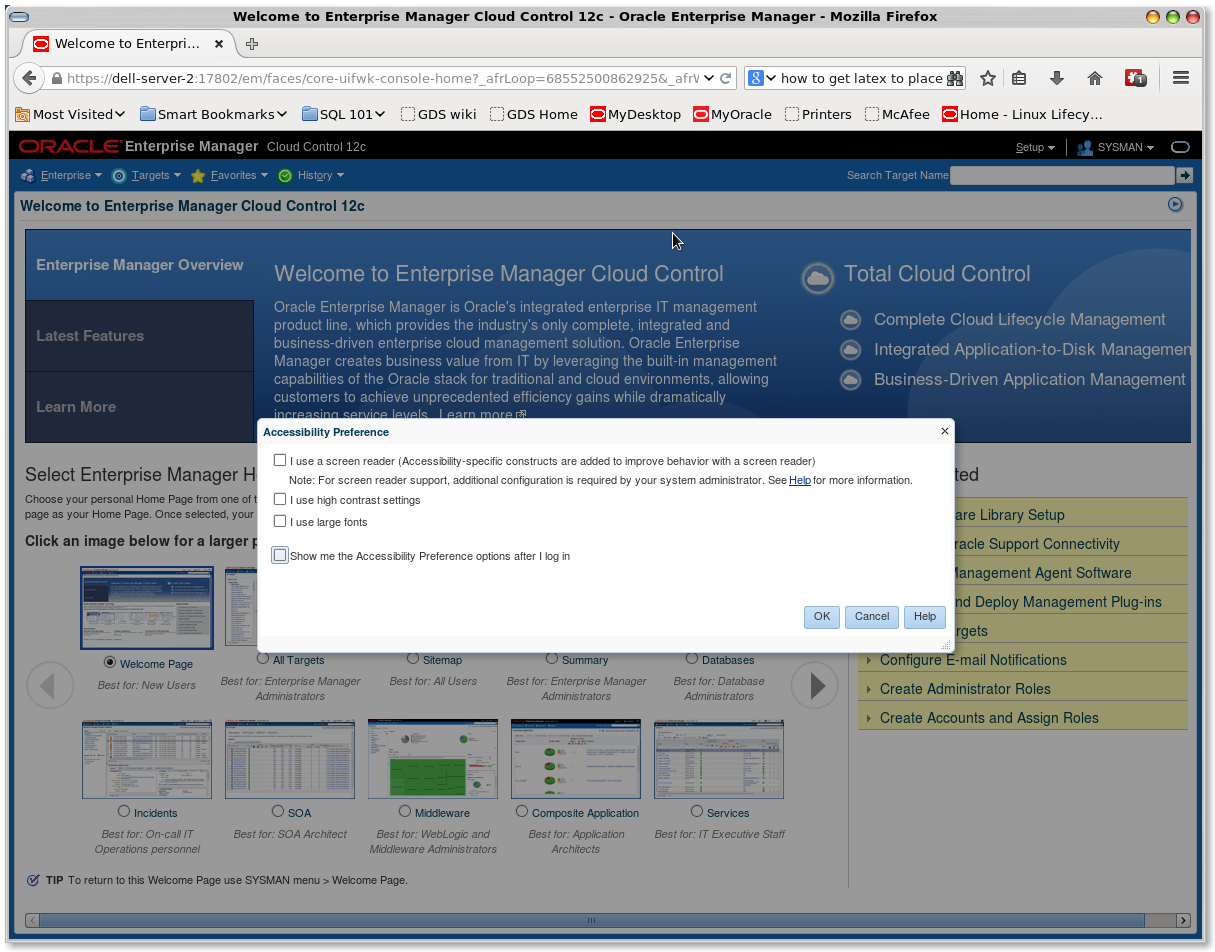
\includegraphics[width=.9\linewidth]{images/Accessibility_Preference.png}
\caption{Accessibility Preferences}
\end{figure}
\clearpage
Select the preferences for you (if any), and then OK. Your preferences are now set up and you will be taken to the 'OEM Welcome' Screen:
\begin{figure}[htb]
\centering
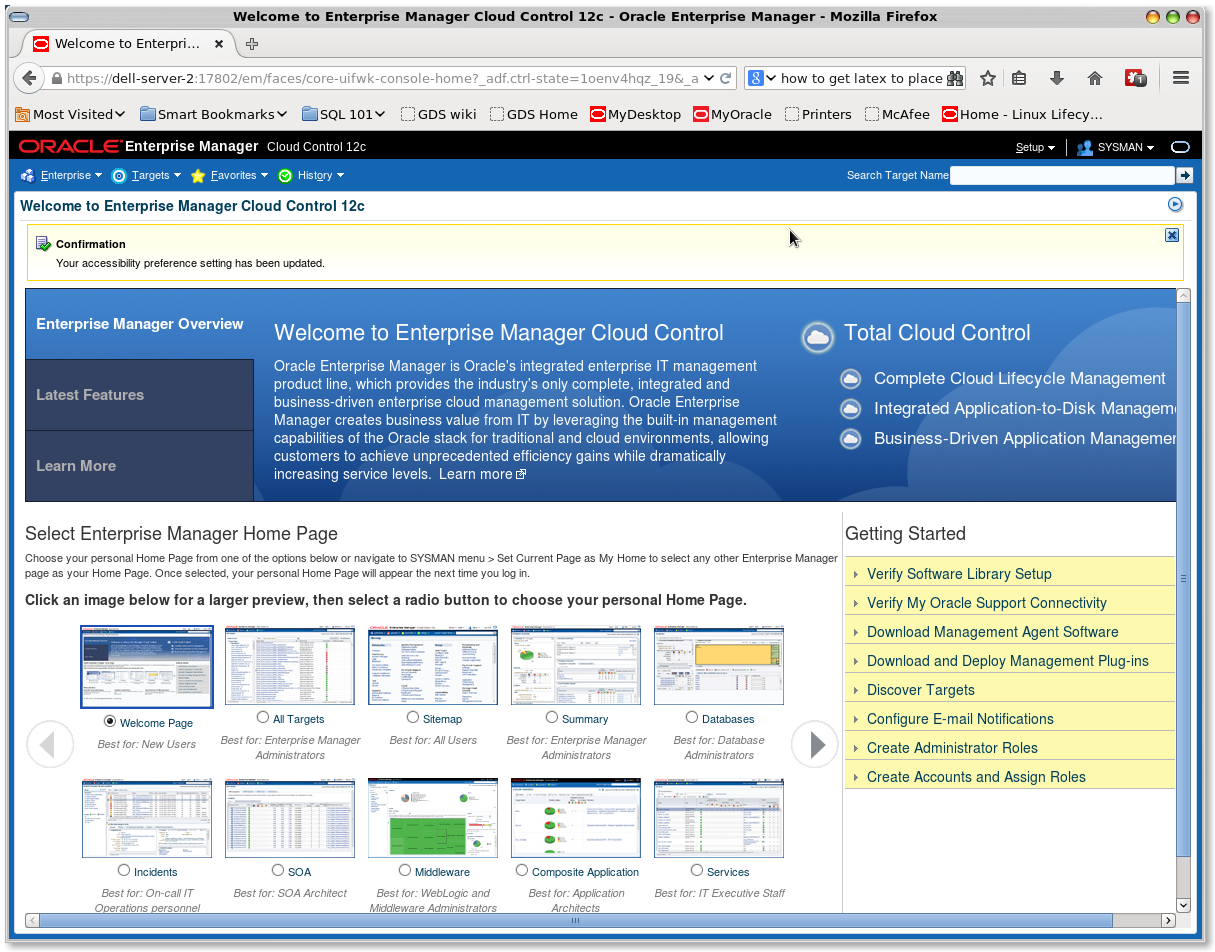
\includegraphics[width=.9\linewidth]{images/OEM_Welcome_Screen.png}
\caption{OEM Welcome Screen}
\end{figure}
\clearpage
(If you need to change these preferences you can do so using the menu Sysman -> Accessibility option)
\begin{figure}[htb]
\centering
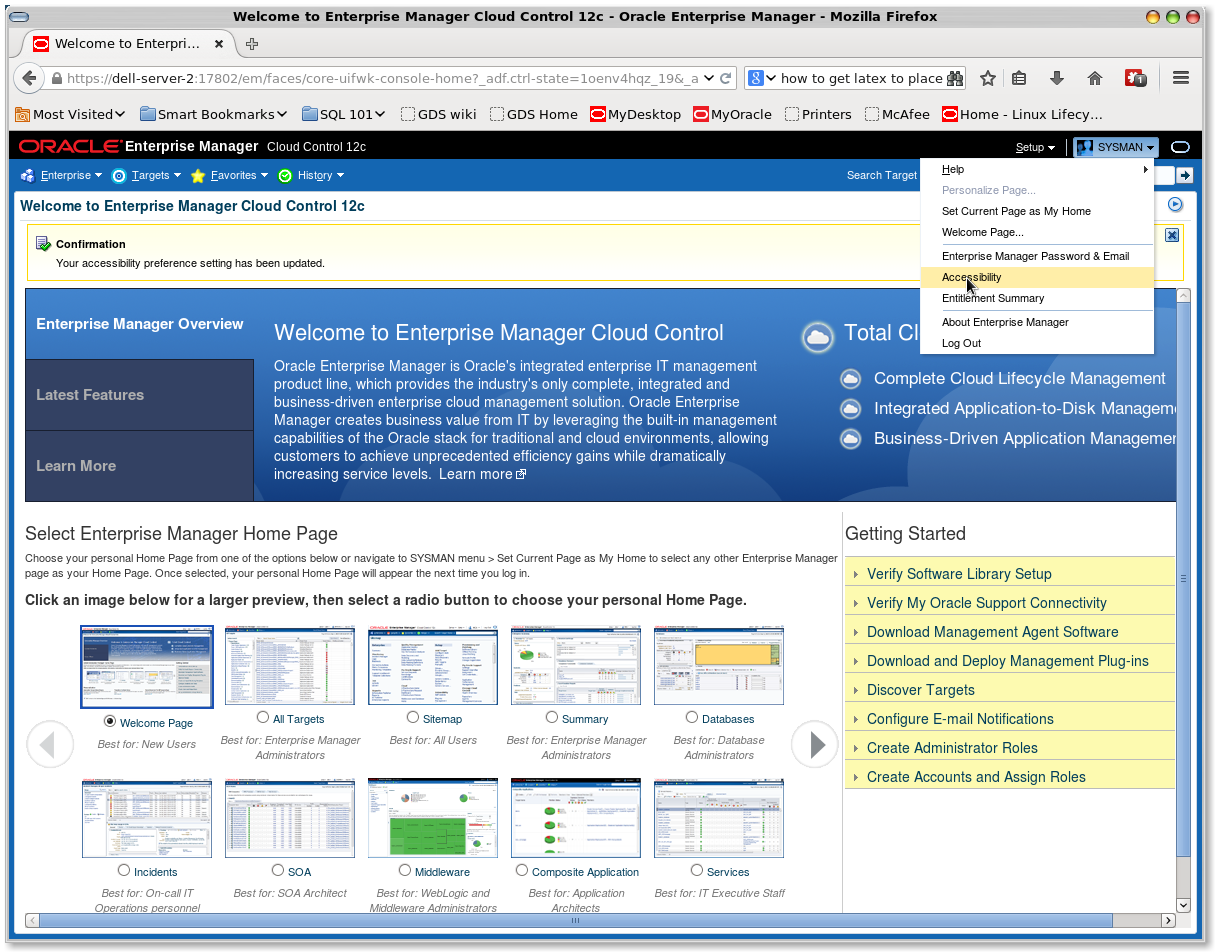
\includegraphics[width=.9\linewidth]{images/OEM_Change_Accessibility.png}
\caption{OEM Change Accessibility Menu}
\end{figure}
\clearpage
\subsection{Software Library}
\label{sec-4-3}
Bare Metal Provisioning, when run using the GUI (it can be run using the command line too), requires that at least two components be setup in the Software Library. These two components are an Operating System Component, and a Disk Component. These components will be referenced later during specific executions of BMP.

Use menu option Enterprise -> Provisioning and Patching -> Software Library to access the Software library:
\begin{figure}[htb]
\centering
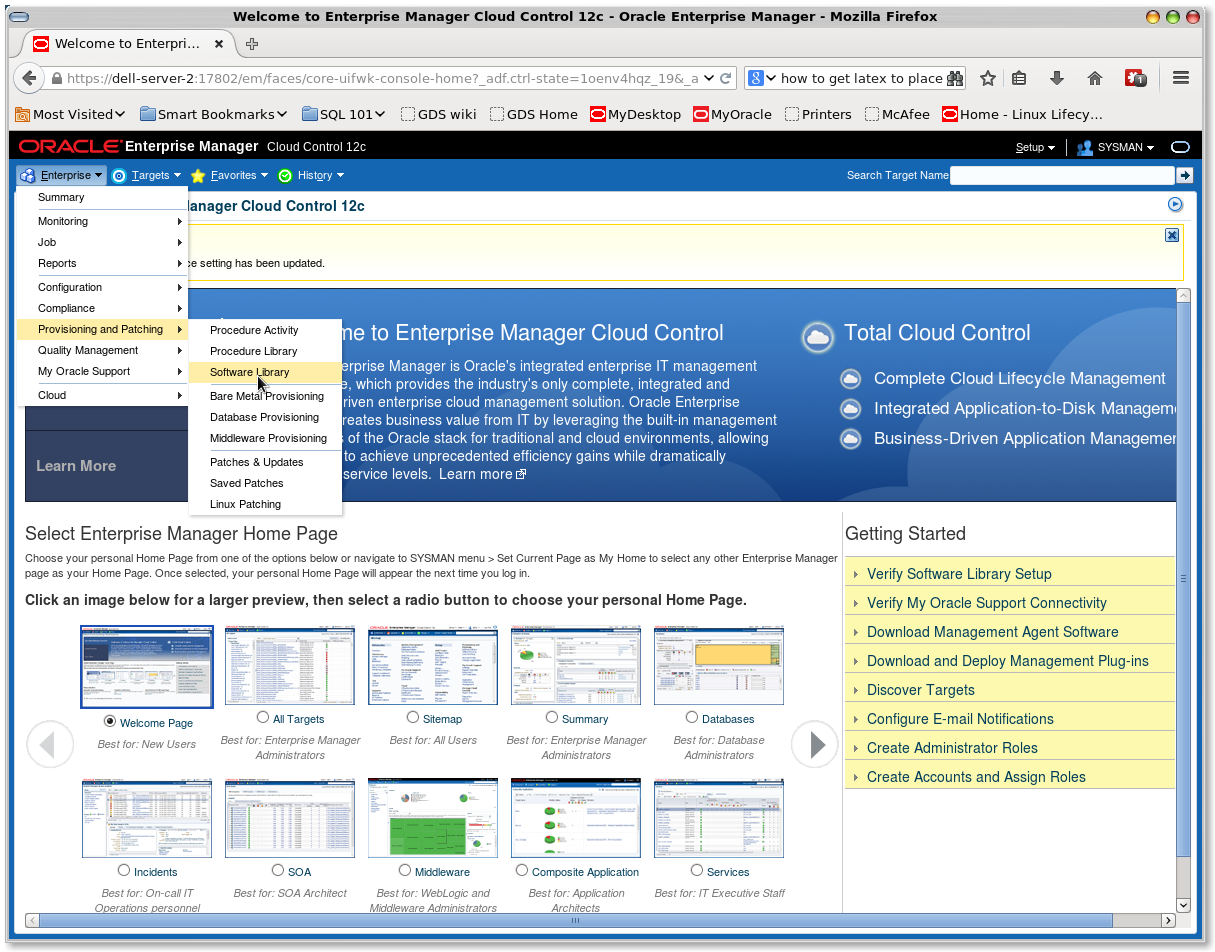
\includegraphics[width=.9\linewidth]{images/OEM_Software_Library_Access.png}
\caption{OEM Software Library Access}
\end{figure}

This will take you to the Software Library:
\begin{figure}[htb]
\centering
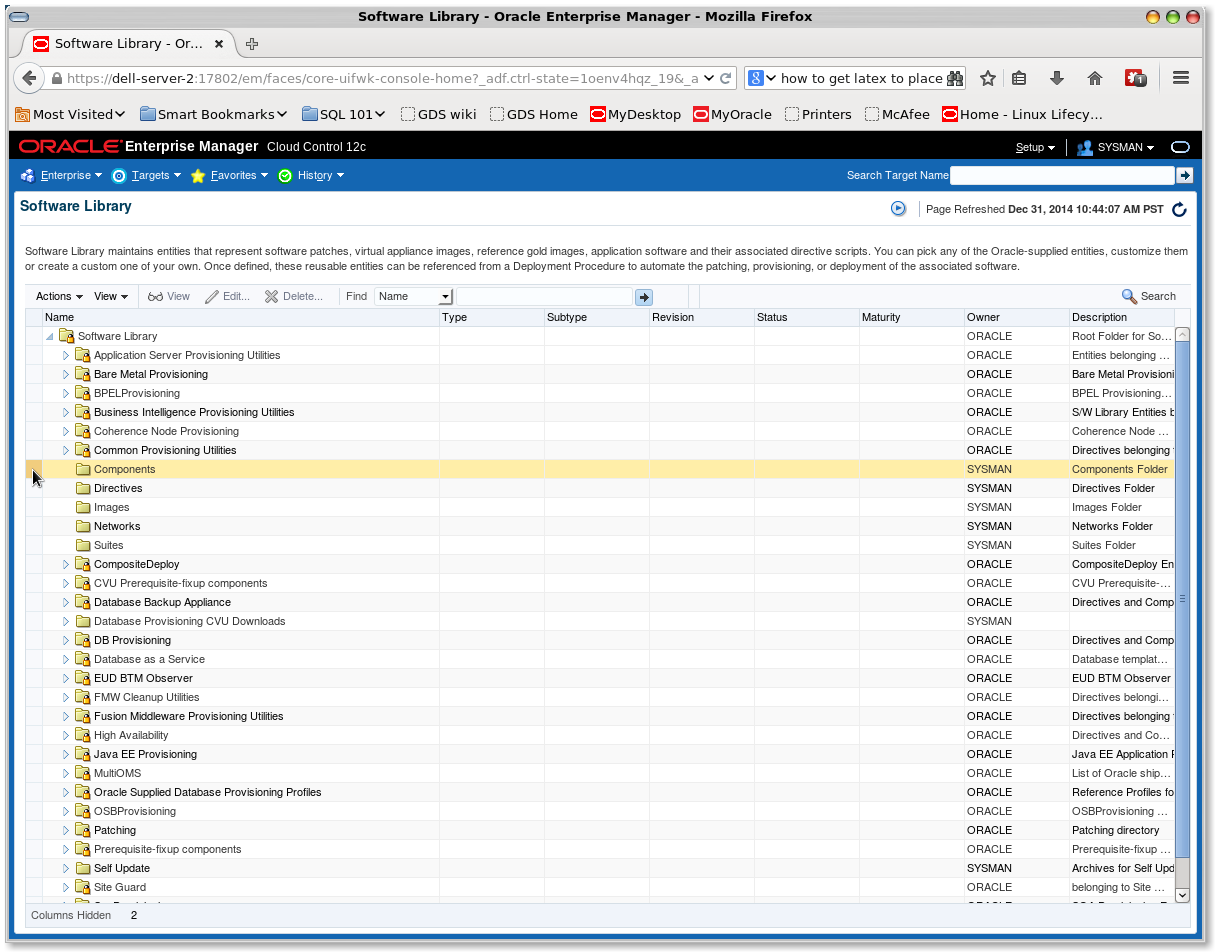
\includegraphics[width=.9\linewidth]{./images/Software_Library_1.png}
\caption{OEM Software Library}
\end{figure}
\clearpage

\subsubsection{Operating System Component}
\label{sec-4-3-1}
To create an Operating System Component right click on the 'Components' line in the Software Library, and select the 'Create Entity -> Bare Metal Provisioning' menu option:
\begin{figure}[htb]
\centering
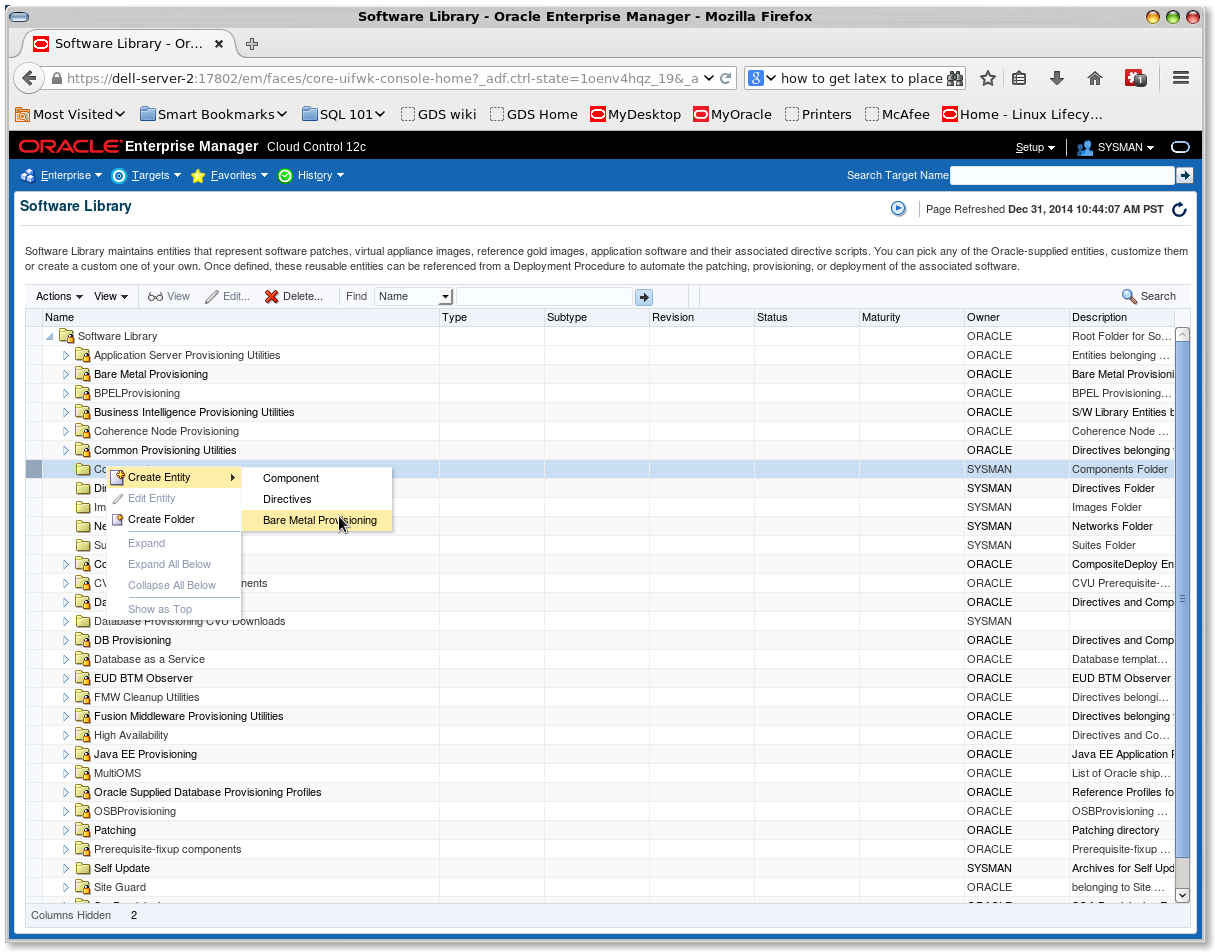
\includegraphics[width=.9\linewidth]{./images/Software_Library_BMP_Menu.png}
\caption{Bare Metal Provisioning Menu Option}
\end{figure}
\clearpage

This will provide a Create Entity pop-up showing the 'Operating System' to be created:
\begin{figure}[htb]
\centering
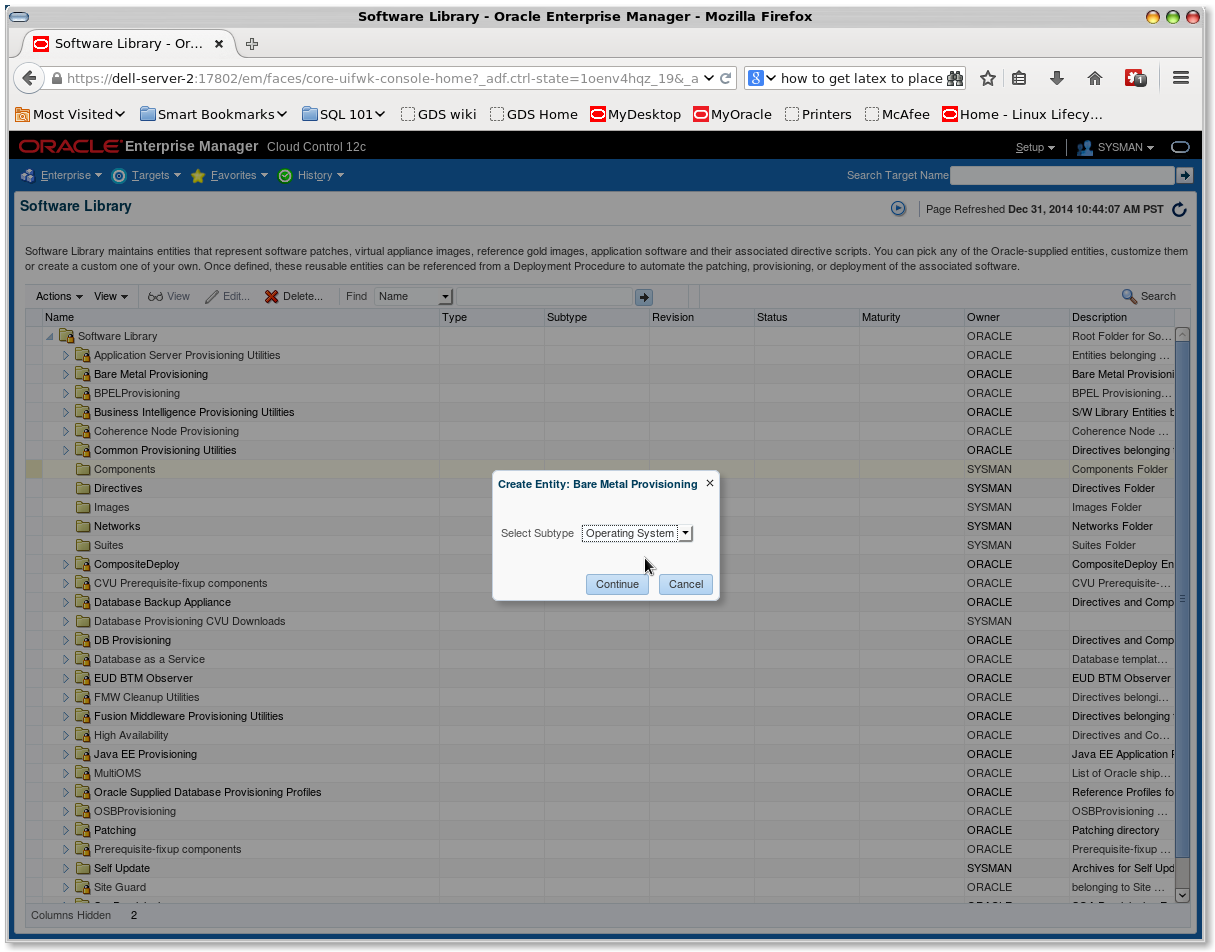
\includegraphics[width=.9\linewidth]{./images/Create_Entity_BMP_OS.png}
\caption{Create Entity (Operating System) pop-up}
\end{figure}
\clearpage

Select 'Continue', and you'll be taken to Step 1 (of 4) of the 'Create Operating System' wizard:
\begin{figure}[htb]
\centering
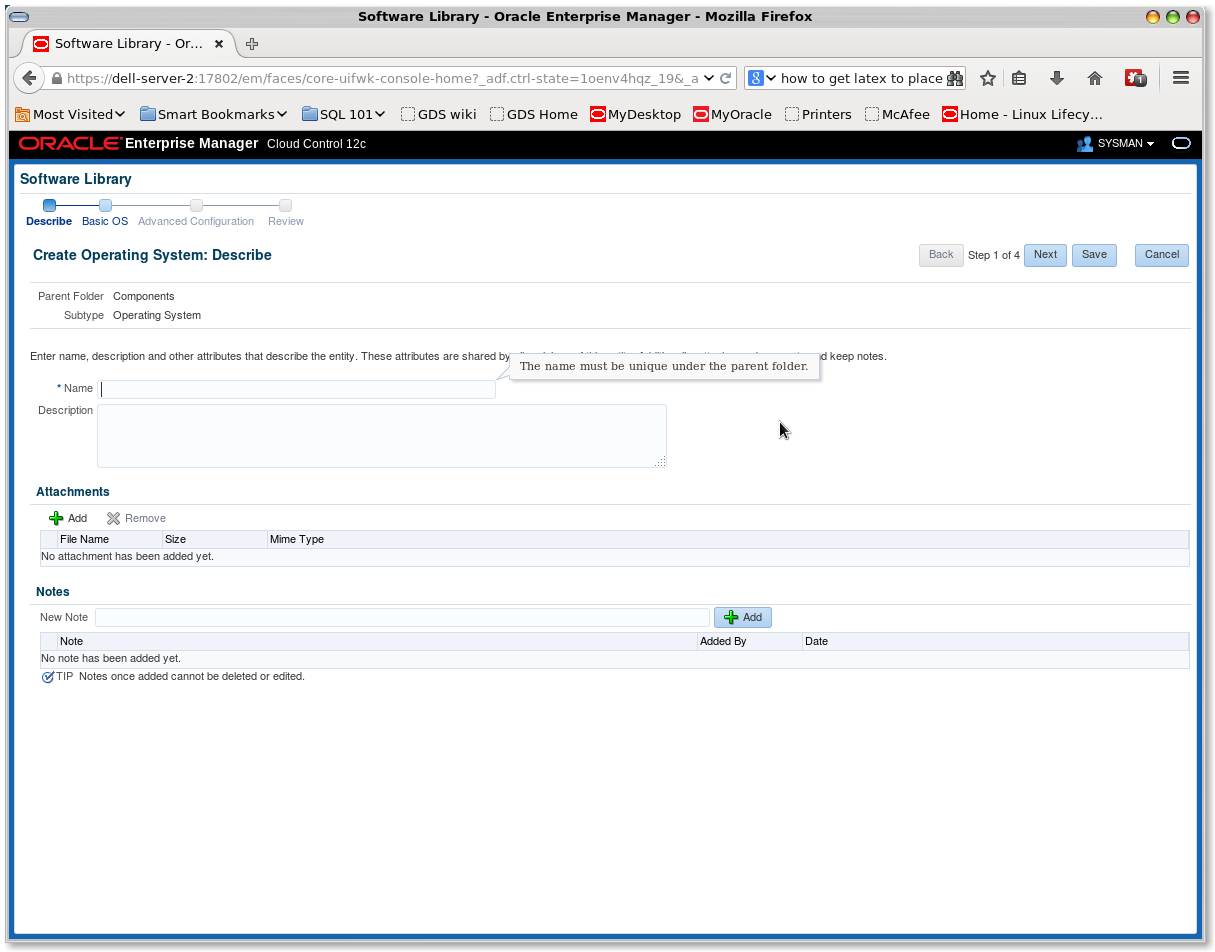
\includegraphics[width=.9\linewidth]{./images/Create_OS_1.png}
\caption{Create OS (Step 1)}
\end{figure}
\clearpage

Provide a name and (optional) description and hit 'Next' to get to Step 2. In Step 2 use the following settings:

\begin{center}
\begin{tabular}{ll}
Item & Value\\
\hline
Timezone & Suit yourself\\
Root password & vagrant\\
Confirm Root Password & vagrant\\
\end{tabular}
\end{center}

(OEM has already been configured with a Named Credential (ROOT$_{\text{NC}}$) with this user/password pair)

Then add a an Operating System User by selecting the 'Add' button. Use the following settings:

\begin{center}
\begin{tabular}{ll}
Item & Value\\
\hline
User Name & oracle\\
Password & oracle\\
Confirm Password & oracle\\
Primary Group & oracle\\
Additional Groups & oinstall\\
 & \\
\end{tabular}
\end{center}

(Again, this user/password combination has already been configured as a Named Credential (ORACLE$_{\text{NC}}$) within OEM)
\begin{figure}[htb]
\centering
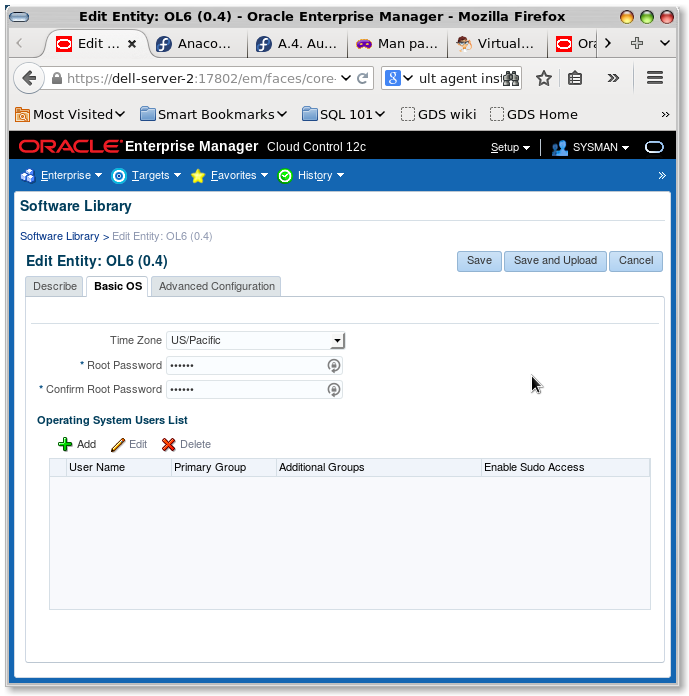
\includegraphics[width=.9\linewidth]{./images/Create_OS_2.png}
\caption{Create OS (Step 2)}
\end{figure}
\clearpage

Hit 'OK' and 'Next' to move to Step 3:

\begin{figure}[htb]
\centering
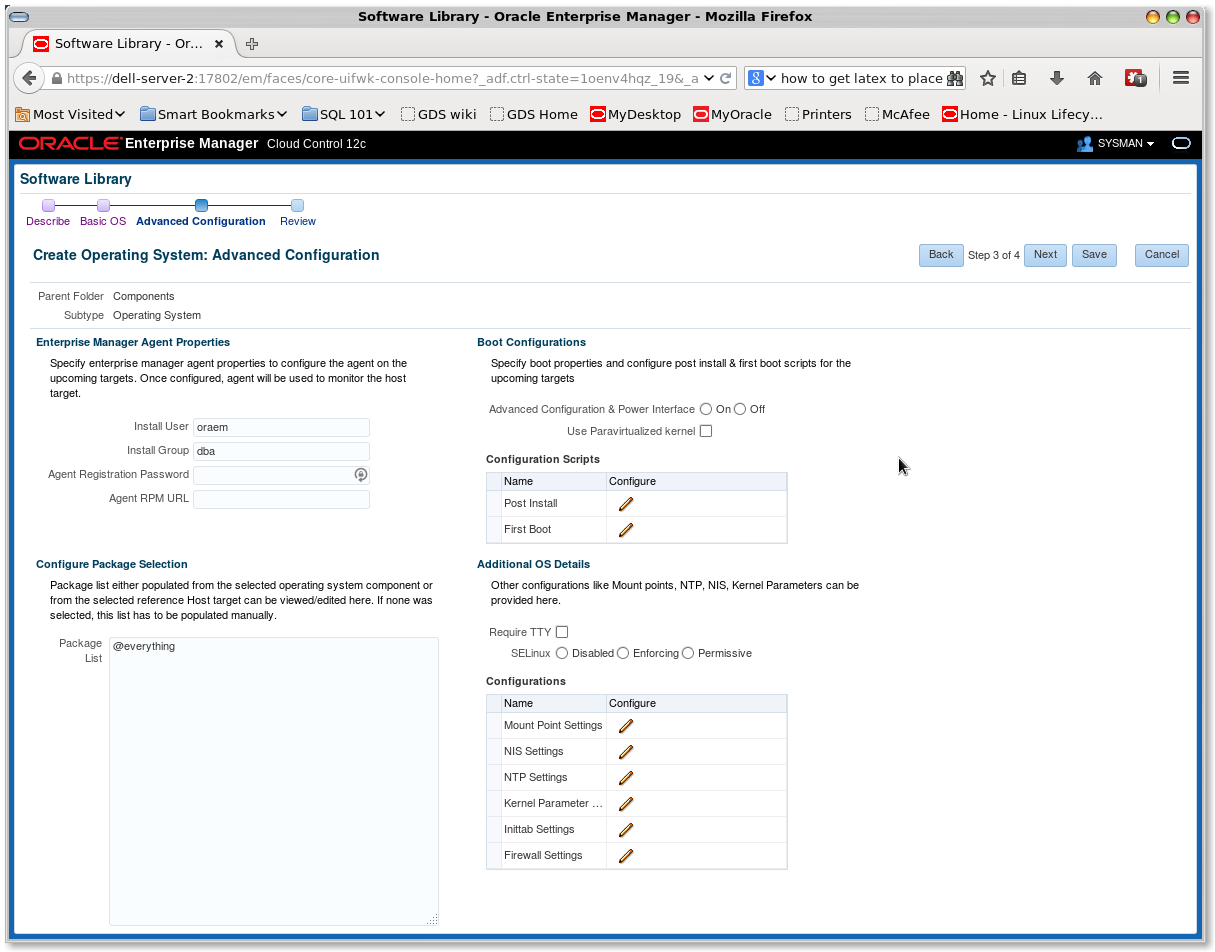
\includegraphics[width=.9\linewidth]{./images/Create_OS_3.png}
\caption{Create OS (Step 3)}
\end{figure}
\clearpage

Set the following Enterprise Manager Agent Properties:
\begin{center}
\begin{tabular}{ll}
Item & Value\\
\hline
Install User & oracle\\
Install Group & oinstall\\
Agent Registration Password & Welcome1\\
\end{tabular}
\end{center}

Change the Package List from \texttt{@everything} to \texttt{@base} - this will greatly reduce the number of packages installed during BMP, thus speeding the process up.

The screen should look like this:
\begin{figure}[htb]
\centering
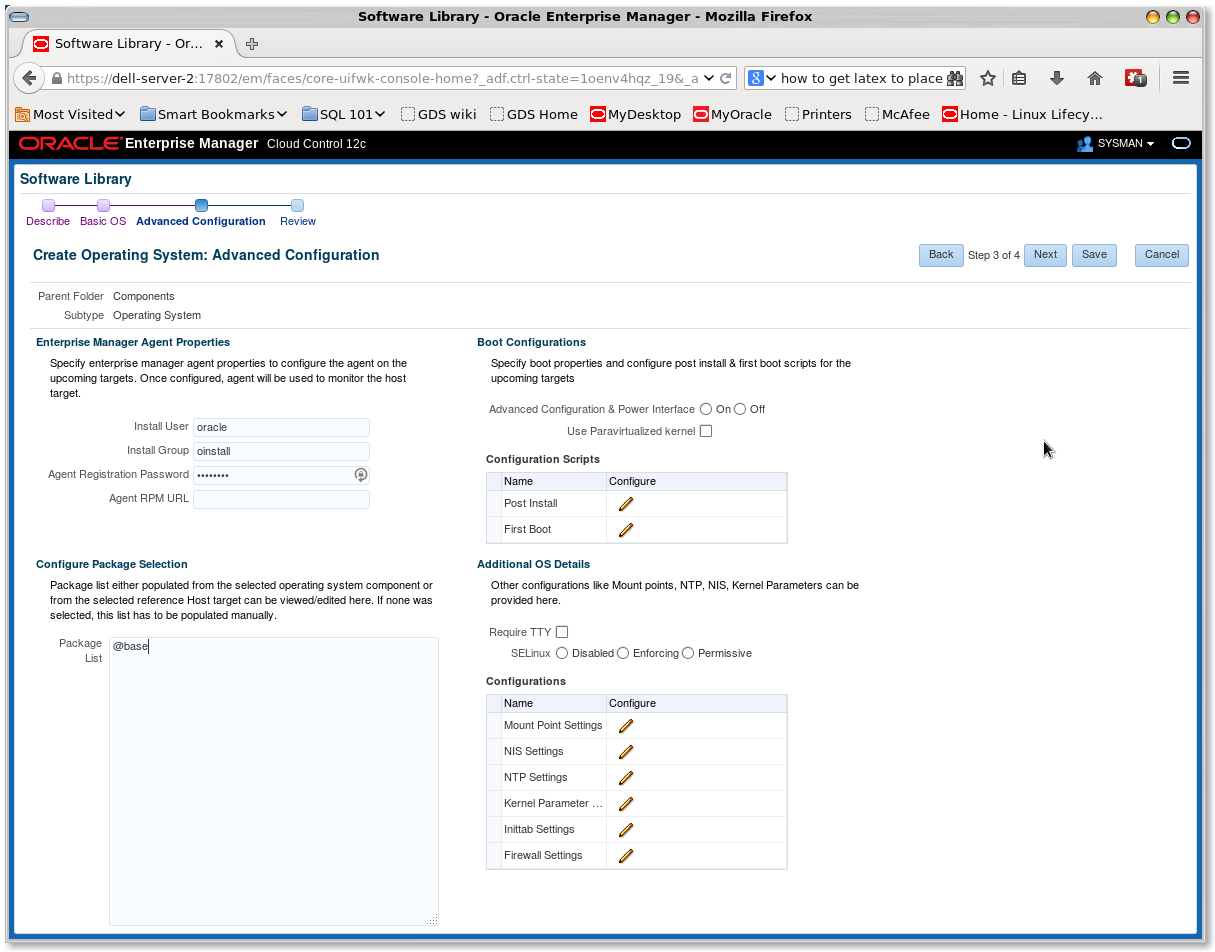
\includegraphics[width=.9\linewidth]{./images/Create_OS_3_Updated.png}
\caption{Create OS (Step 3) With Properties Updated}
\end{figure}
\clearpage

Hit 'Next' to get to Step 4 (Review):
\begin{figure}[htb]
\centering
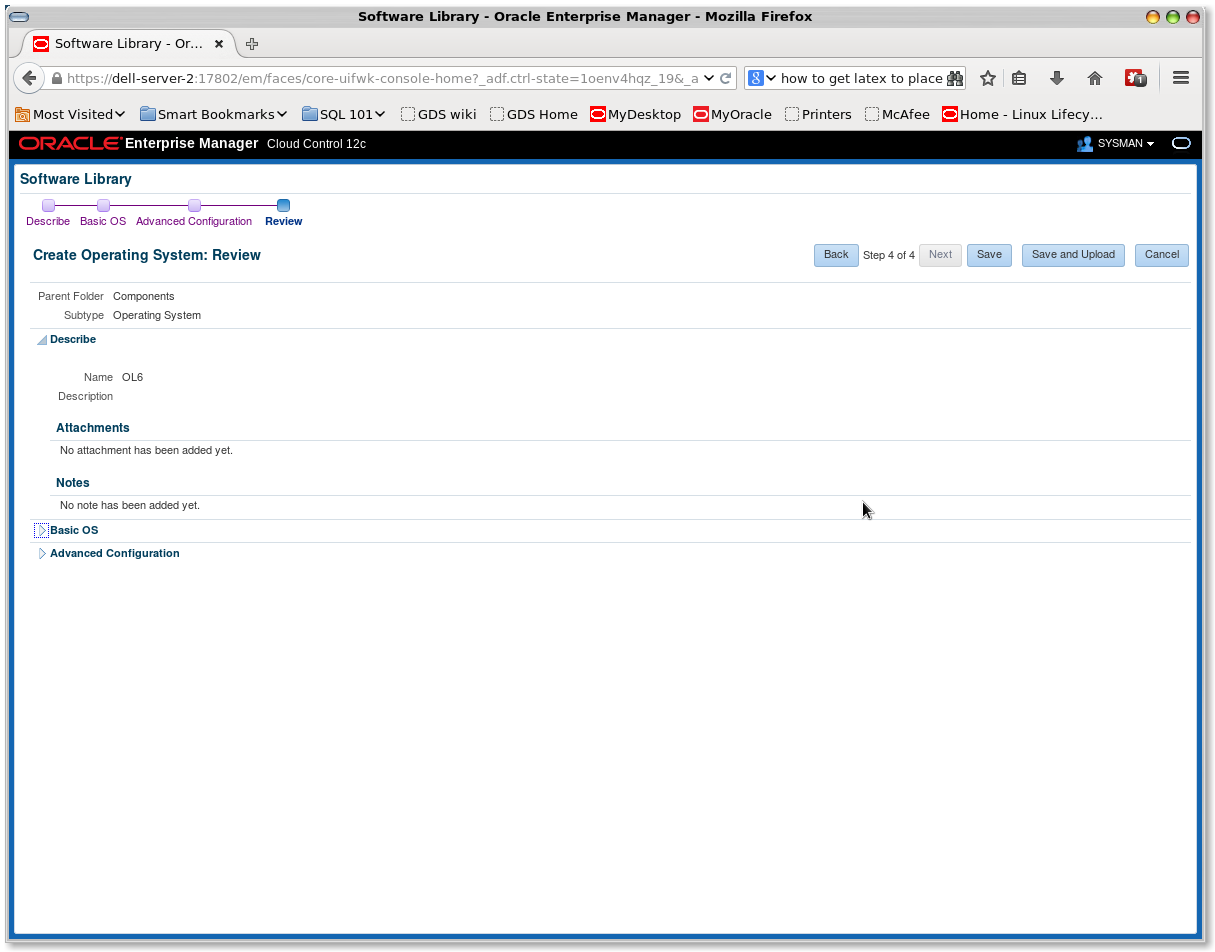
\includegraphics[width=.9\linewidth]{./images/Create_OS_4.png}
\caption{Create OS (Step 4)}
\end{figure}
\clearpage

Review the settings (you can go back and change them if you think you made a mistake). When satisfied hit 'Save and Upload' to save this component into the Software Library. 
\begin{figure}[htb]
\centering
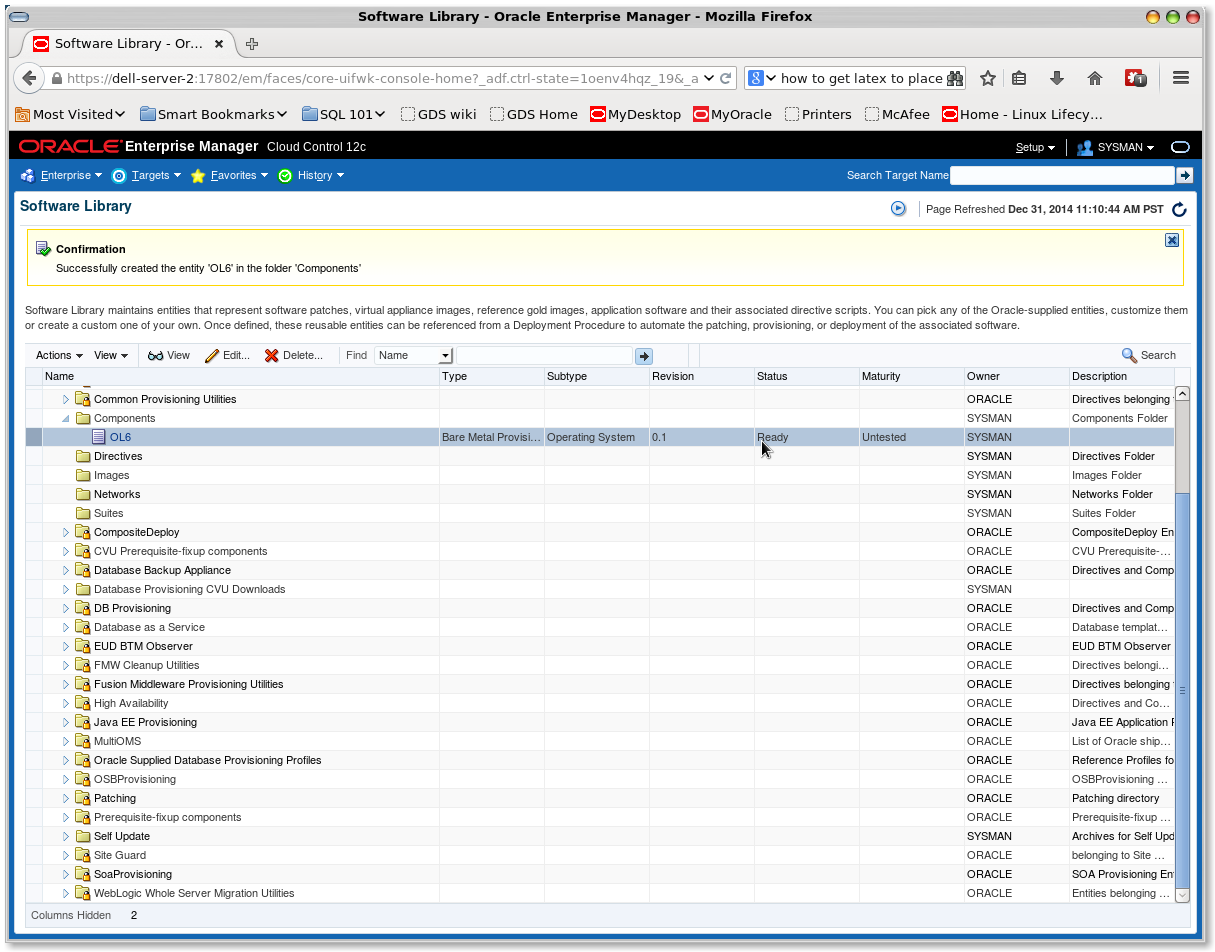
\includegraphics[width=.9\linewidth]{./images/Create_OS_Completed.png}
\caption{Create OS Completed}
\end{figure}
\clearpage
\subsubsection{Disk Component}
\label{sec-4-3-2}
Create a Disk Component by right clicking on the 'Components' line in the Software Library and selecting the 'Create Entity -> Bare Metal Provisioning' menu option:
\begin{figure}[htb]
\centering
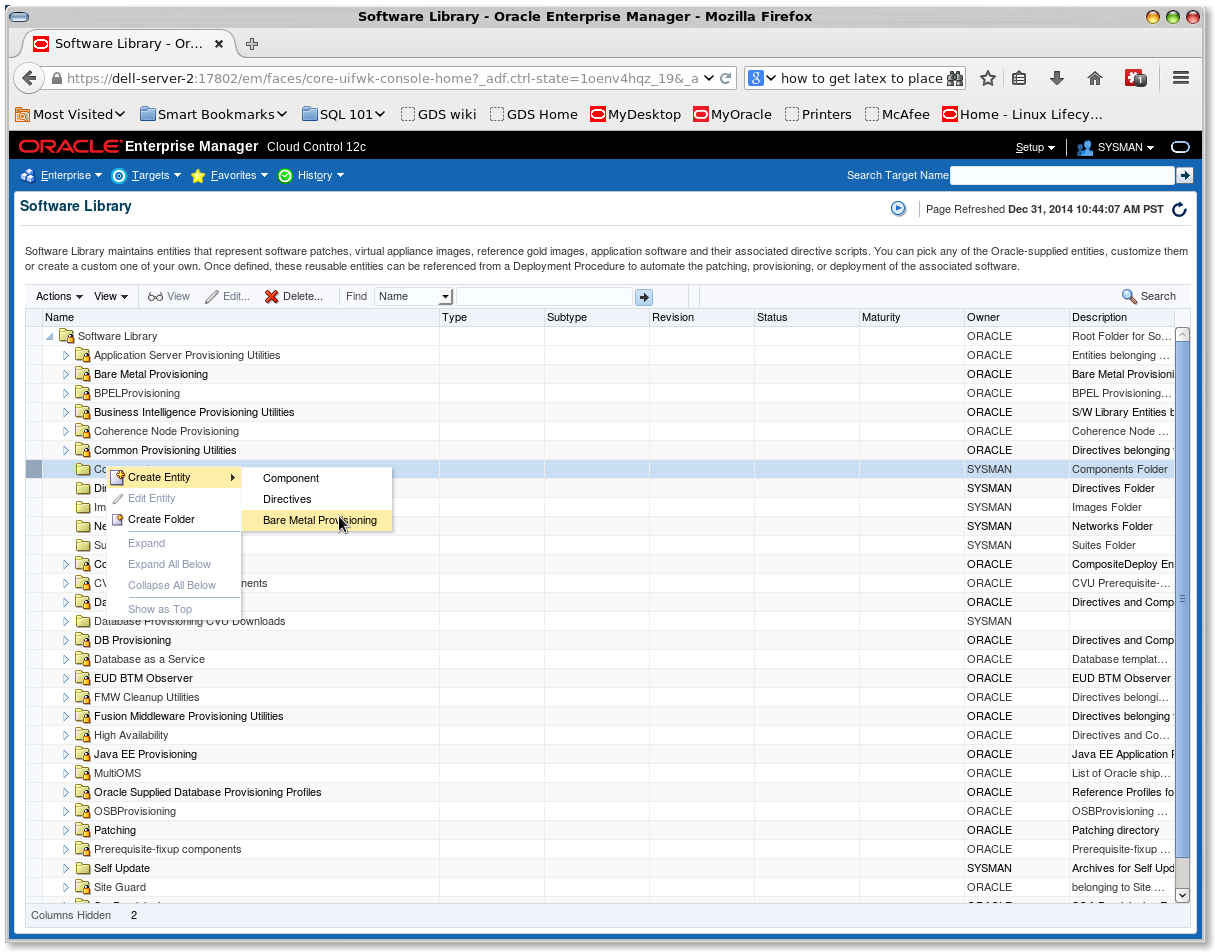
\includegraphics[width=.9\linewidth]{./images/Software_Library_BMP_Menu.png}
\caption{Bare Metal Provisioning Menu Option}
\end{figure}
\clearpage

This will provide a Create Entity pop-up showing the 'Operating System' to be created. Change the selection to 'Disk Layout':
\begin{figure}[htb]
\centering
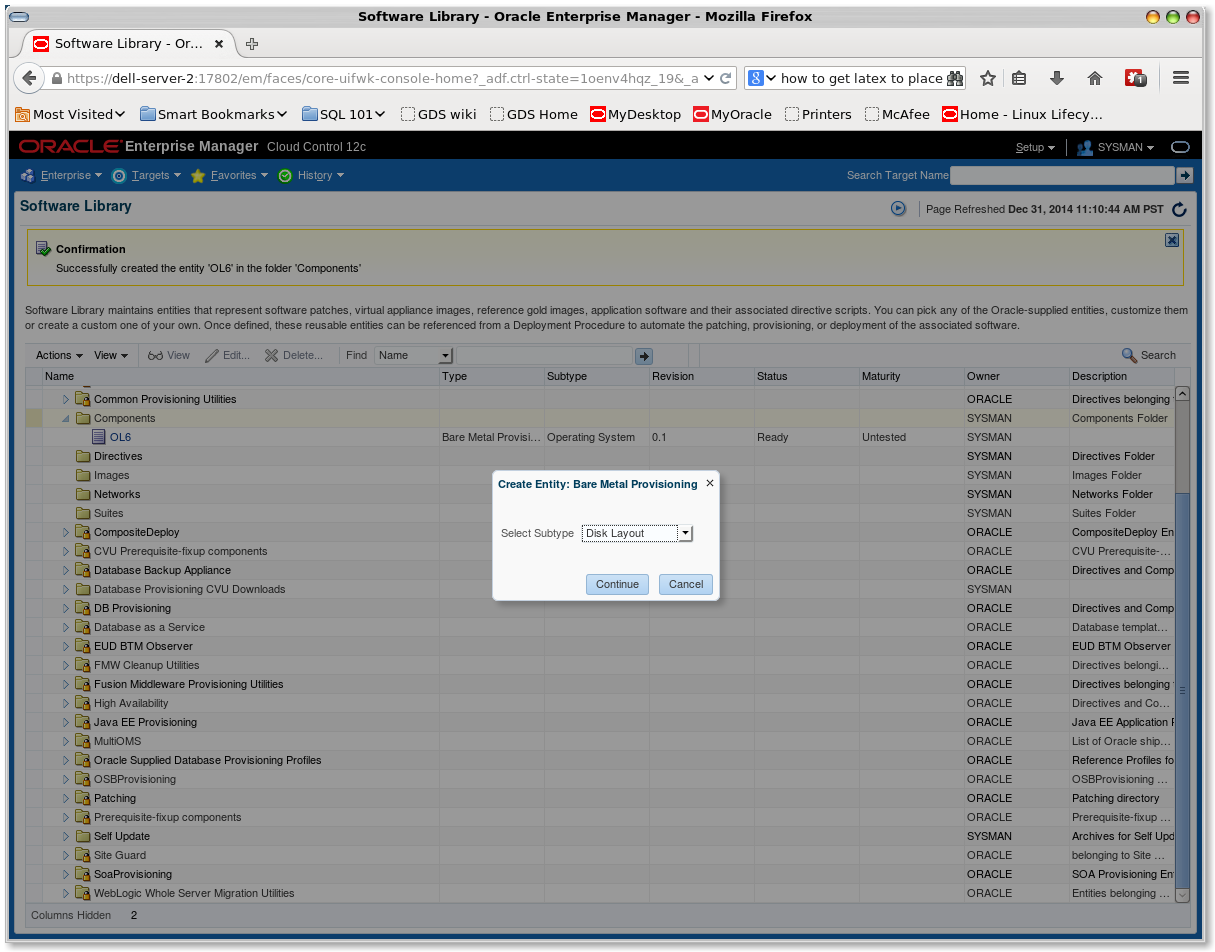
\includegraphics[width=.9\linewidth]{./images/Create_Entity_BMP_DL.png}
\caption{Create Entity (Disk Layout) pop-up}
\end{figure}
\clearpage

Hit 'Continue' to go to Step 1 (of 3) in the Create Disk Layout wizard.
\begin{figure}[htb]
\centering
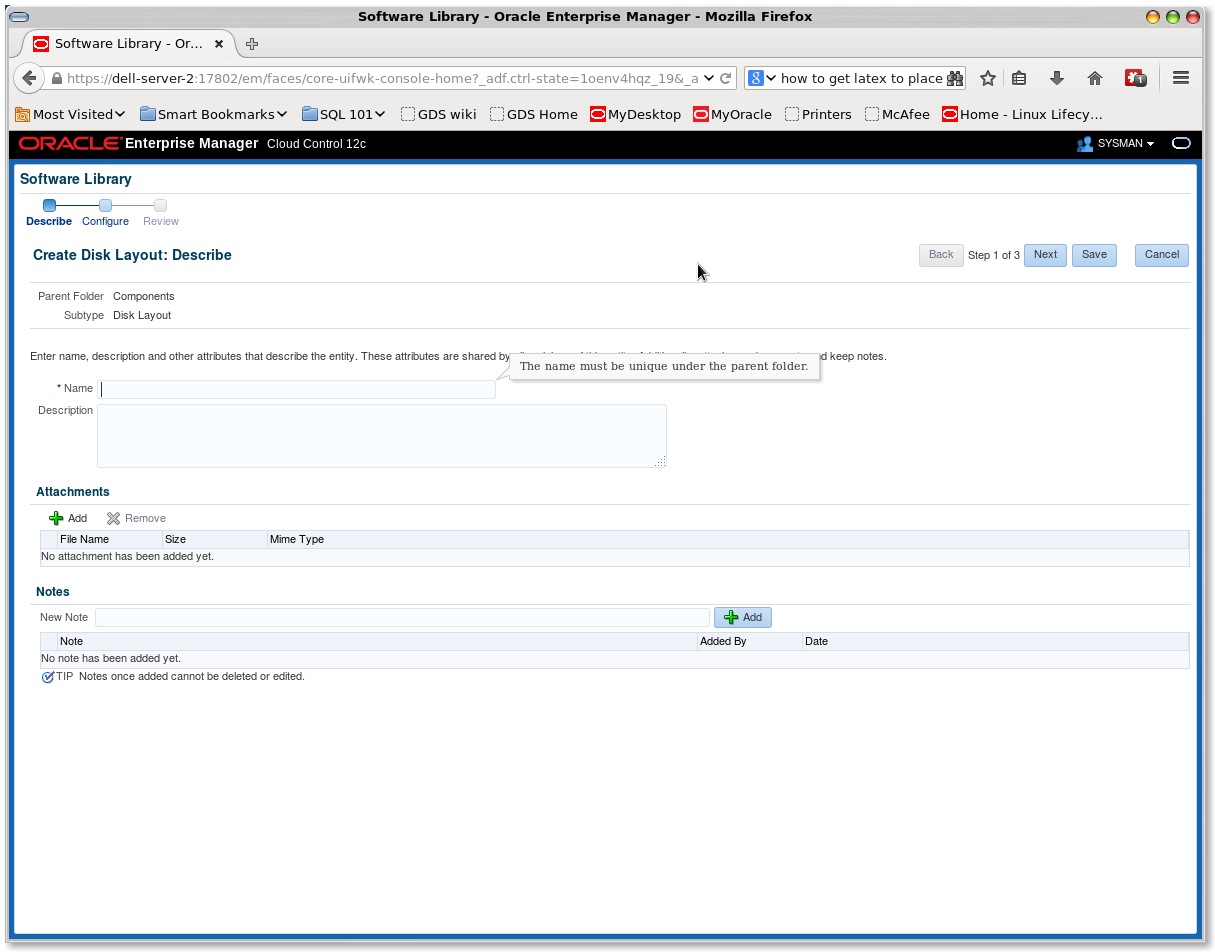
\includegraphics[width=.9\linewidth]{./images/Create_DL_1.png}
\caption{Create Disk Layout (Step 1)}
\end{figure}
\clearpage

Provide a name and (optional) description and hit 'Next' to move to Step 2 of the Disk Layout wizard:
\begin{figure}[htb]
\centering
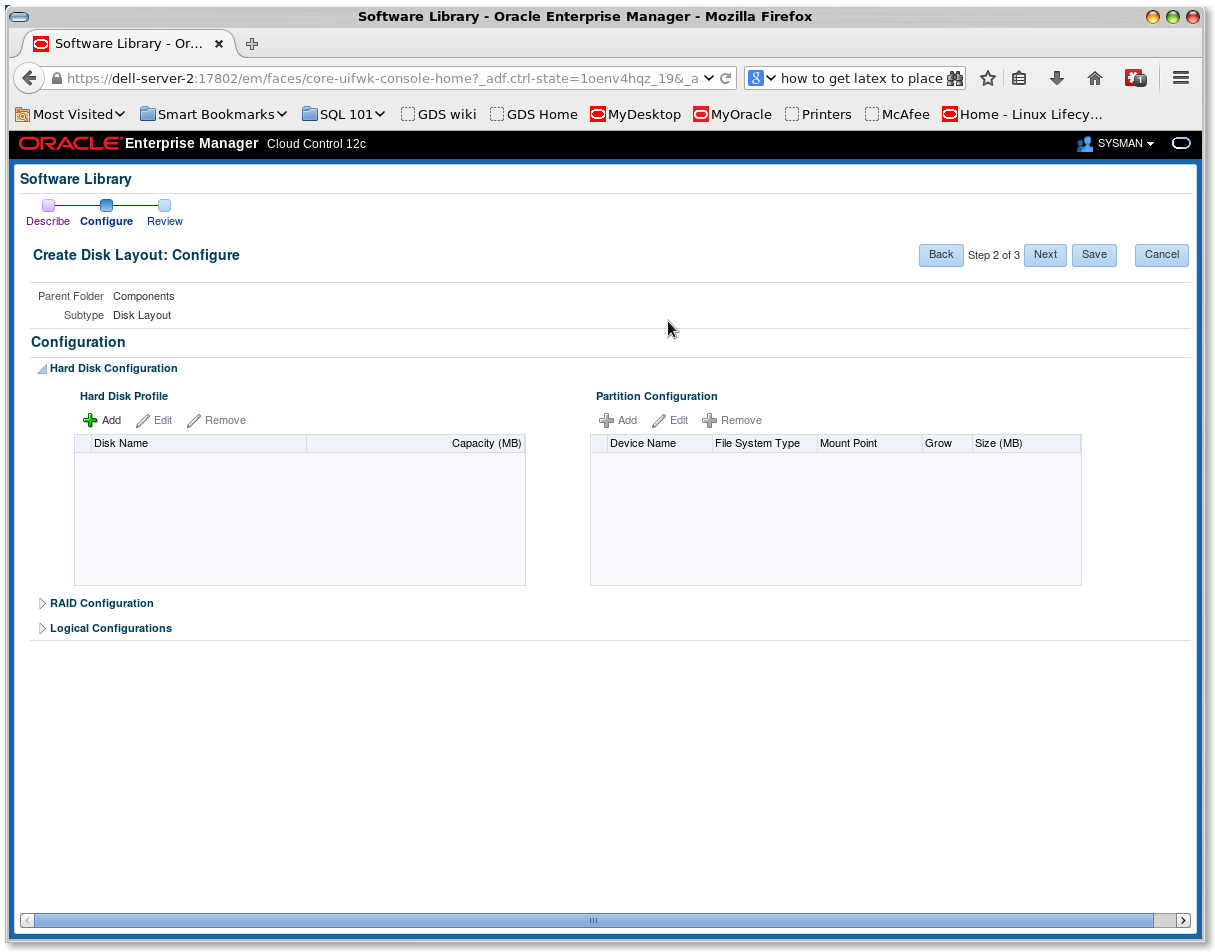
\includegraphics[width=.9\linewidth]{./images/Create_DL_2.png}
\caption{Create Disk Layout (Step 2)}
\end{figure}
\clearpage

Add a Disk Profile by selecting the appropriate 'Add' button, and create a disk named \texttt{sda} with a size of 15360 MB (15GB):
\begin{figure}[htb]
\centering
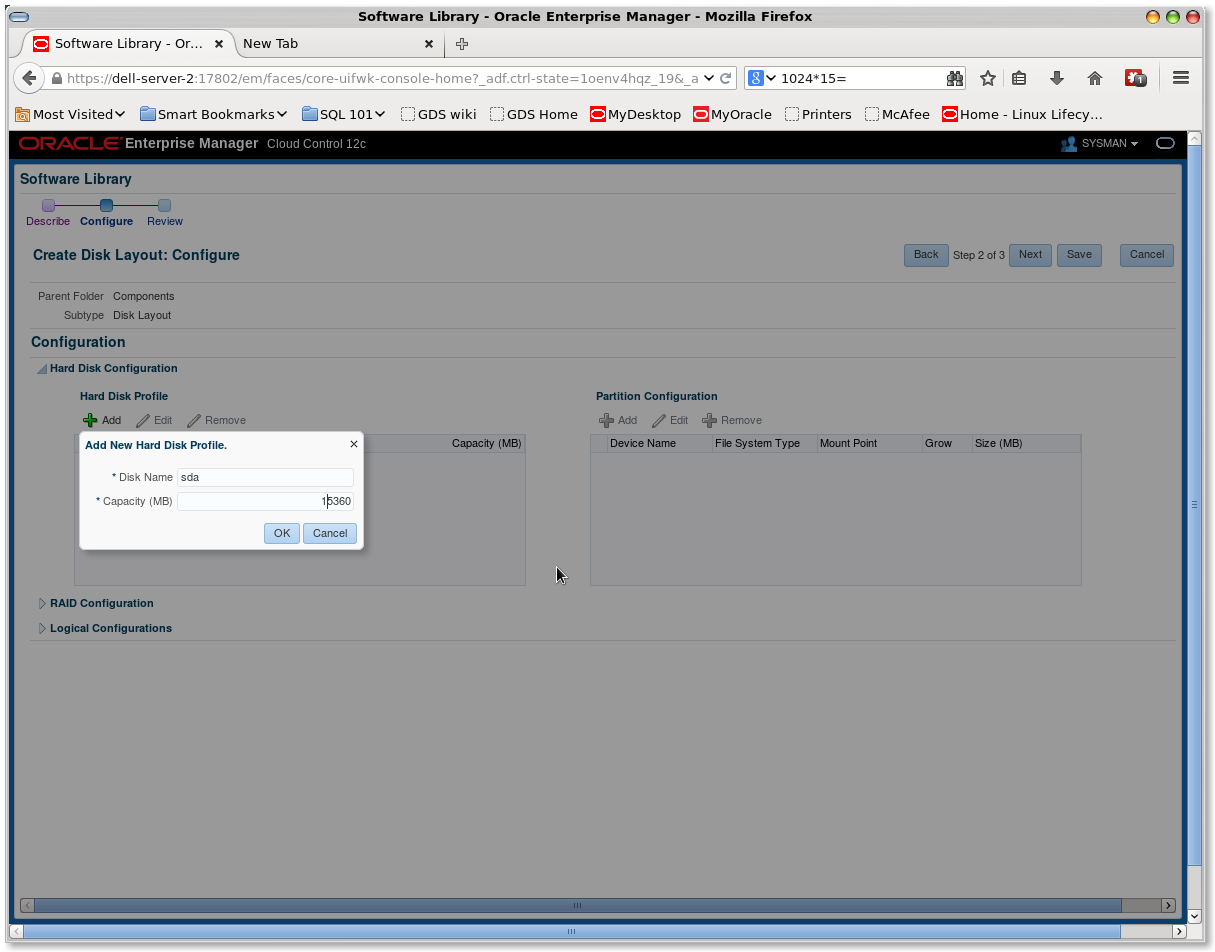
\includegraphics[width=.9\linewidth]{./images/Add_New_Hard_Disk_Profile.png}
\caption{Add New Hard Disk Profile}
\end{figure}
\clearpage

Add three partitions using the 'Add' button under 'Partition Configuration', configured thus:

\begin{center}
\begin{tabular}{llllr}
Device Name & File System Type & Mount Point & Grow & Size (MB)\\
\hline
/dev/sda0 & ext3 & /boot & false & 200\\
/dev/sda1 & swap & swap & false & 1024\\
/dev/sda2 & ext3 & / & true & 1\\
\end{tabular}
\end{center}
\begin{figure}[htb]
\centering
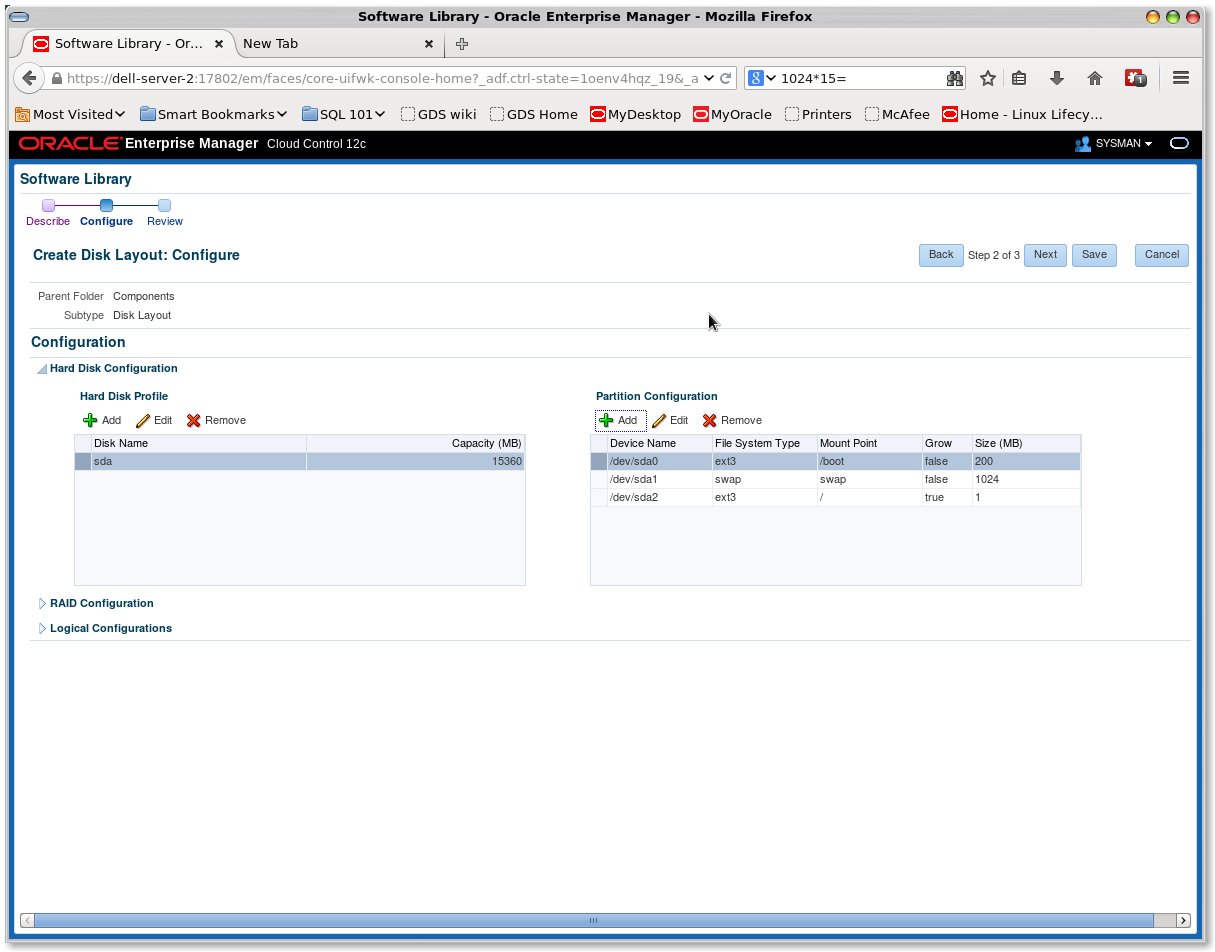
\includegraphics[width=.9\linewidth]{./images/Partition_Configuration.png}
\caption{Partition Configuration}
\end{figure}
\clearpage

More complex disk layouts are possible, but for simplicity's sake we'll go with this basic layout. Select 'Next' to move to Step 3 of the Disk Layout wizard. Expanding the 'Configure' subsection will show the configuration that has been completed so far. Review it, go back to make changes if necessary:
\begin{figure}[htb]
\centering
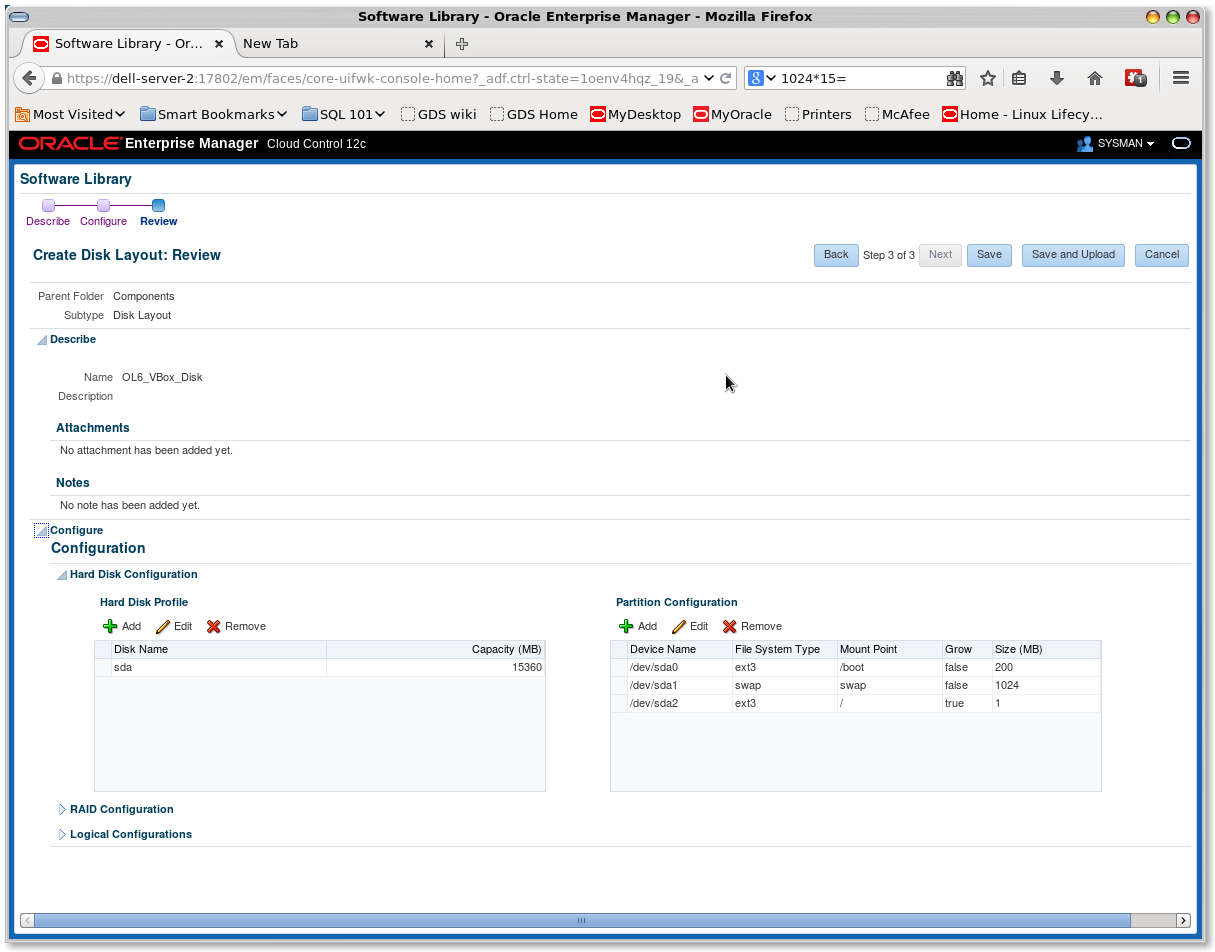
\includegraphics[width=.9\linewidth]{./images/Create_DL_3.png}
\caption{Create Disk Layout (Step 3)}
\end{figure}  
\clearpage

Select 'Save and Upload' to be taken back to the Software Library:
\begin{figure}[htb]
\centering
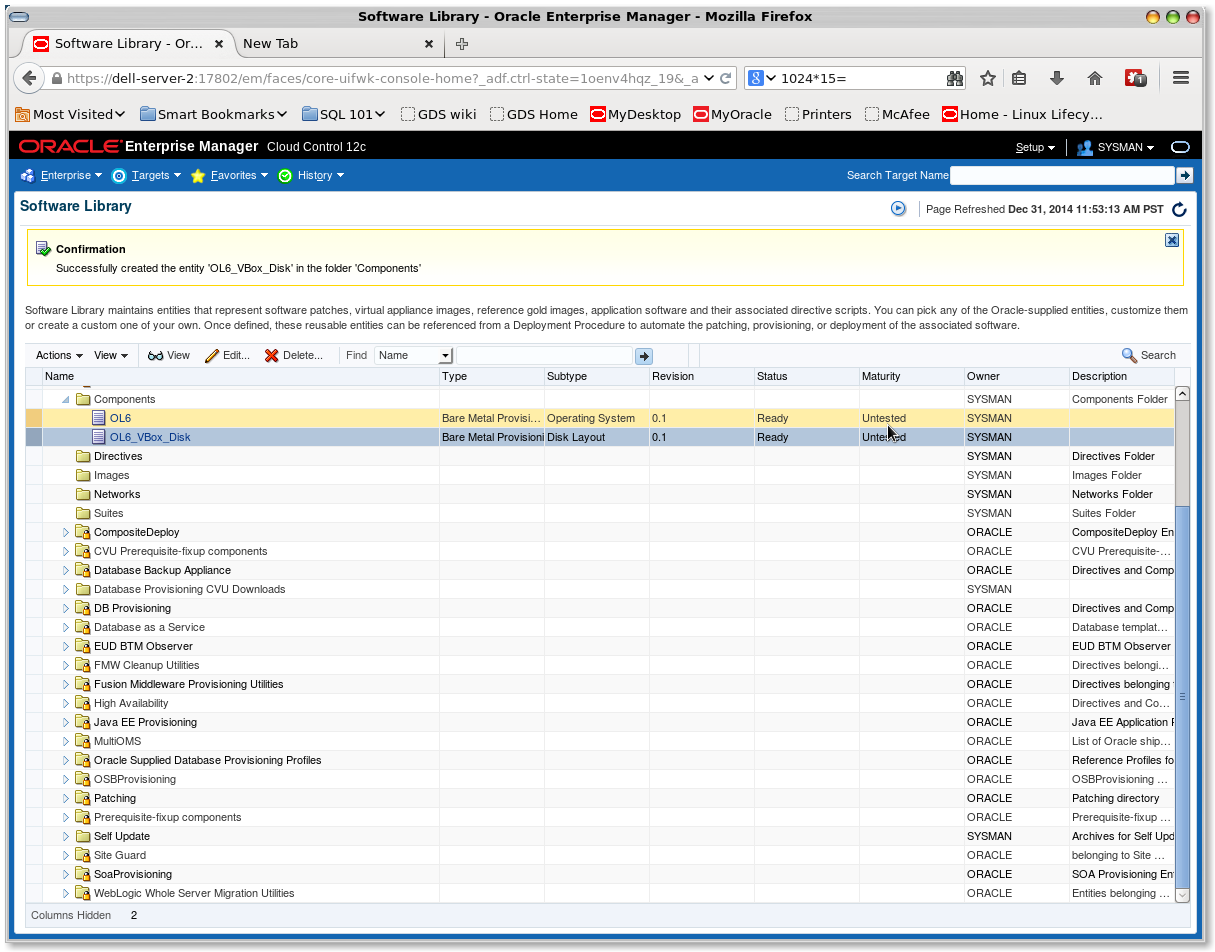
\includegraphics[width=.9\linewidth]{./images/Create_DL_Completed.png}
\caption{Create Disk Layout Component Completed}
\end{figure}
\clearpage
\subsection{Bare Metal Provisioning Infrastructure}
\label{sec-4-4}
Access the Bare Metal Provisioning wizard by selecting the Enterprise -> Provisioning and Patching -> Bare Metal Provisioning menu option:
\begin{figure}[htb]
\centering
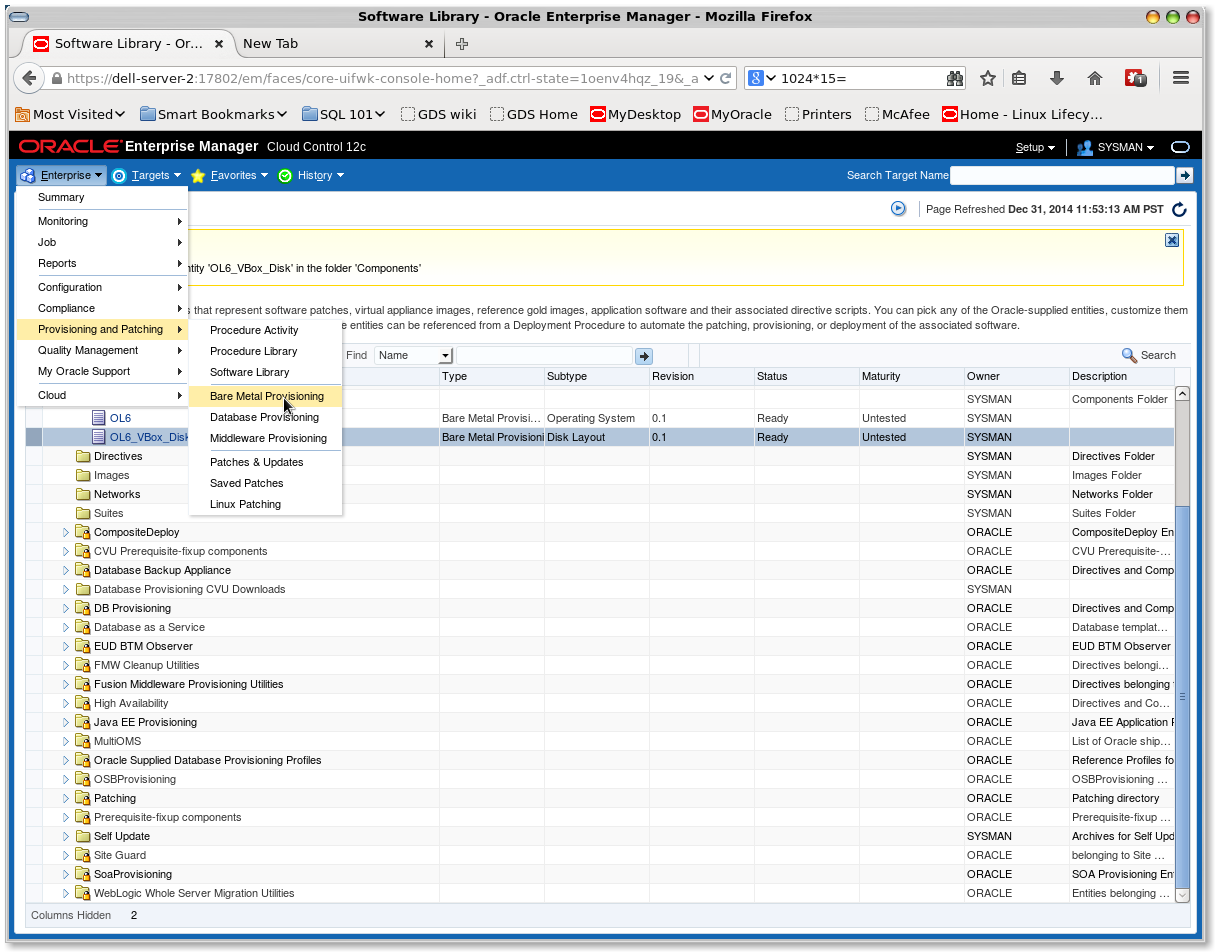
\includegraphics[width=.9\linewidth]{./images/BMP_Menu_Option.png}
\caption{Bare Metal Provisioning Menu Option:}
\end{figure}
\clearpage
This will take you to the initial BMP screen:
\begin{figure}[htb]
\centering
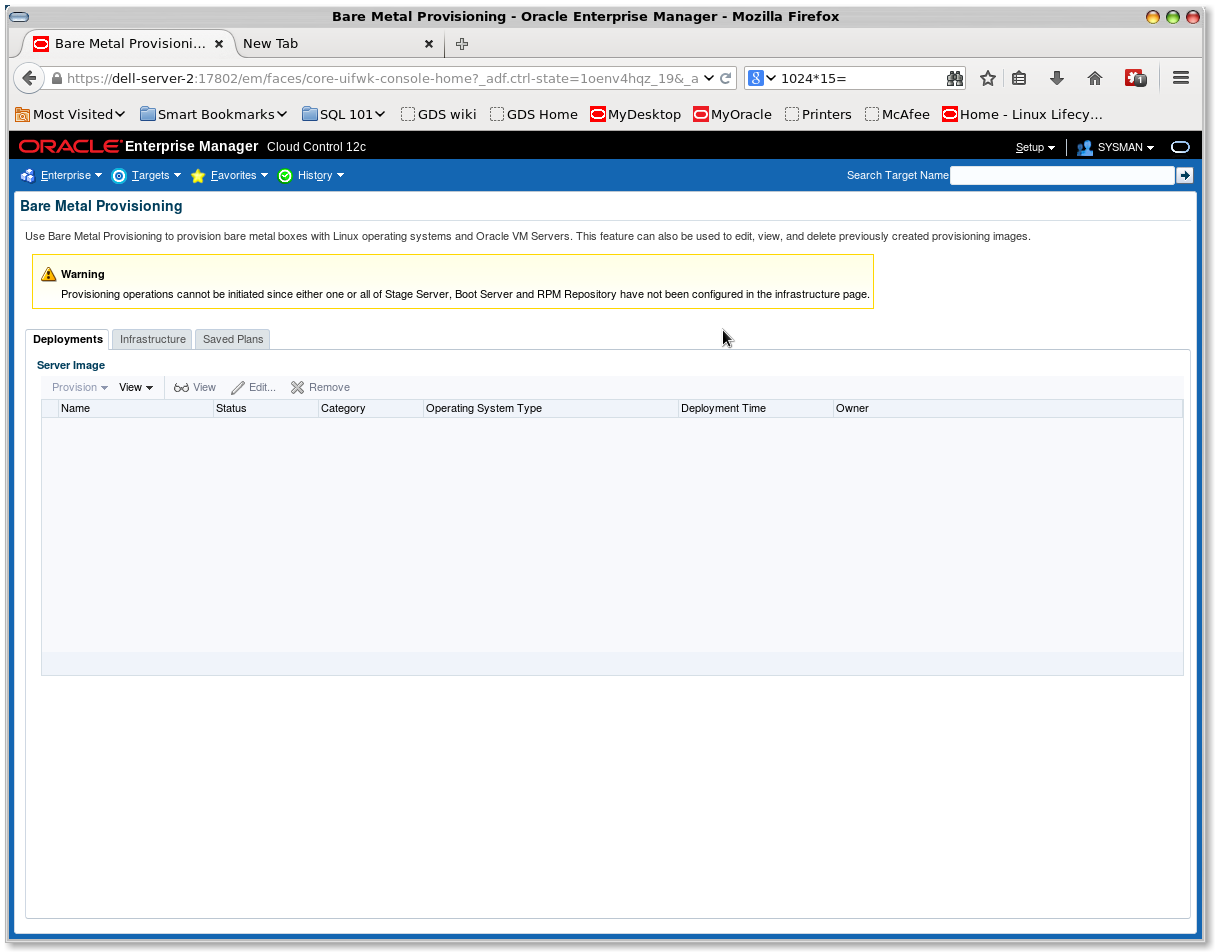
\includegraphics[width=.9\linewidth]{./images/BMP_1.png}
\caption{BMP Initial Screen}
\end{figure}
\clearpage
As indicated on that initial page no BMP can occur because one or more parts of the infrastructure have not been configured. 
Select the 'Infrastructure' tab to begin the setup:
\begin{figure}[htb]
\centering
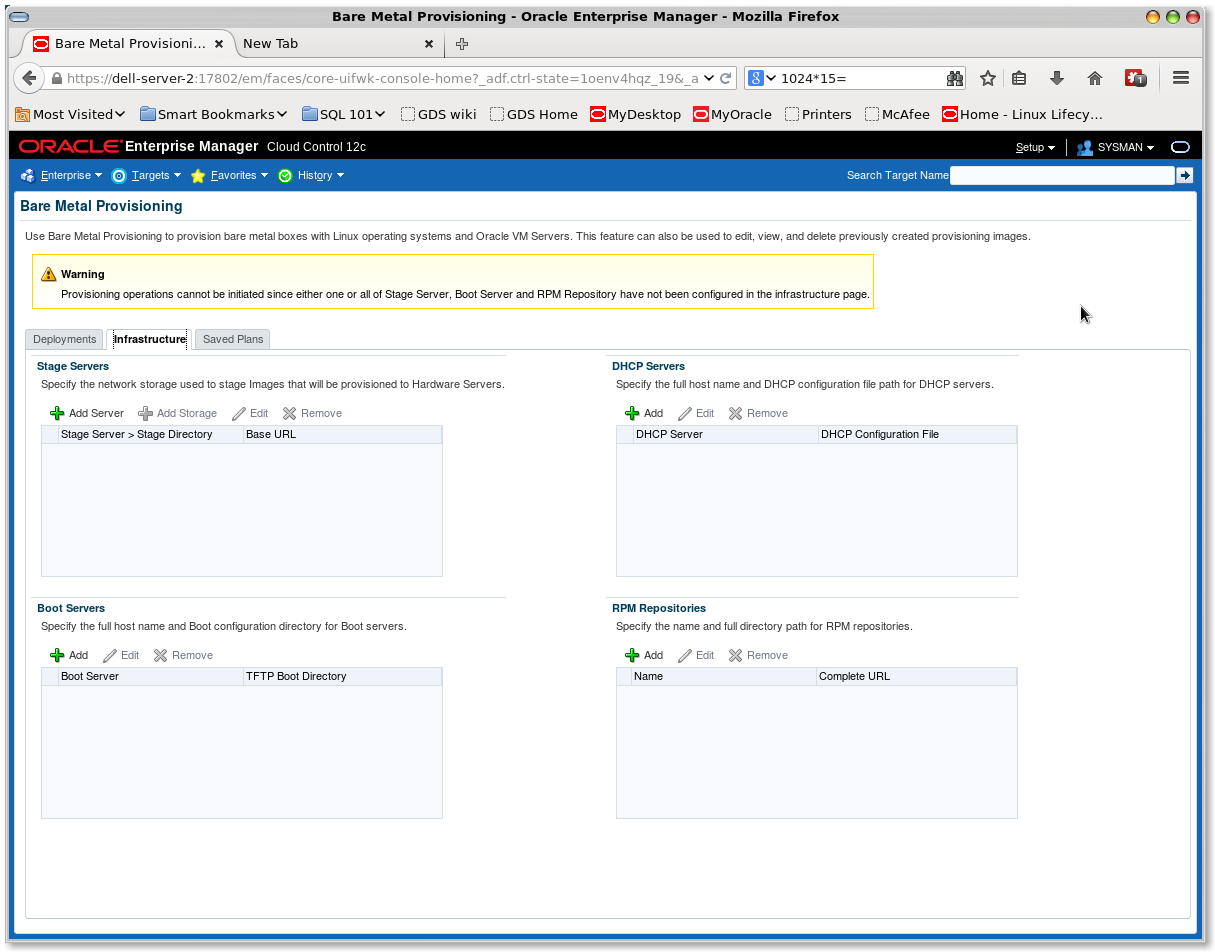
\includegraphics[width=.9\linewidth]{./images/Infra_1.png}
\caption{Infrastructure Wizard}
\end{figure}
\clearpage

Add a Stage Server by selecting the appropriate 'Add' button to open up the 'Add Stage Server' wizard:
\begin{figure}[htb]
\centering
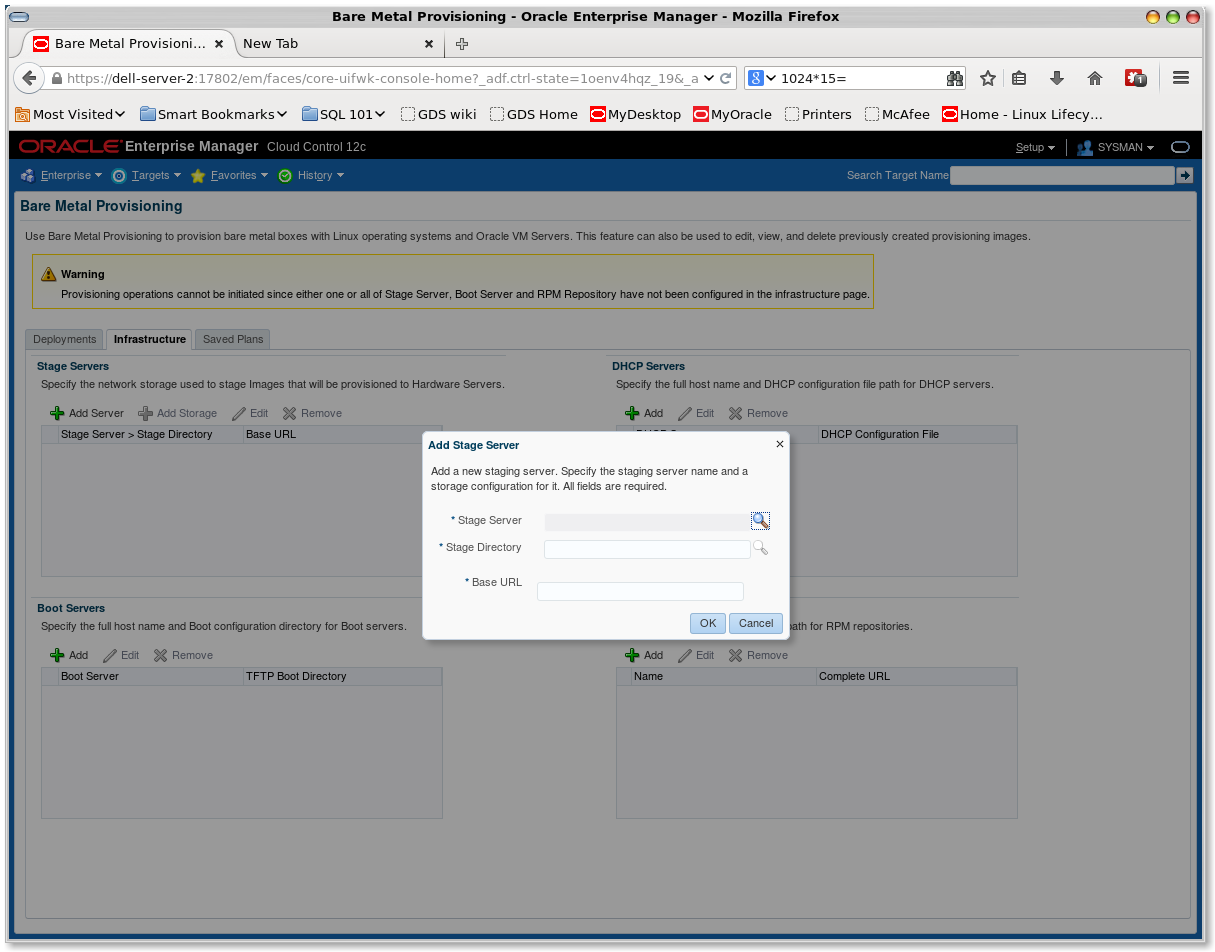
\includegraphics[width=.9\linewidth]{./images/Server_Add_1.png}
\end{figure}
\clearpage

Select the stage server by clicking on the magnifying glass on the right and then using the Select Targets wizard\footnote{Alternatively, for the Stage Directory property, by selecting the magnifying glass on the 'Stage Directory' line you can open up the 'Remote File Browser' to select the directory using a wizard}:
\begin{figure}[htb]
\centering
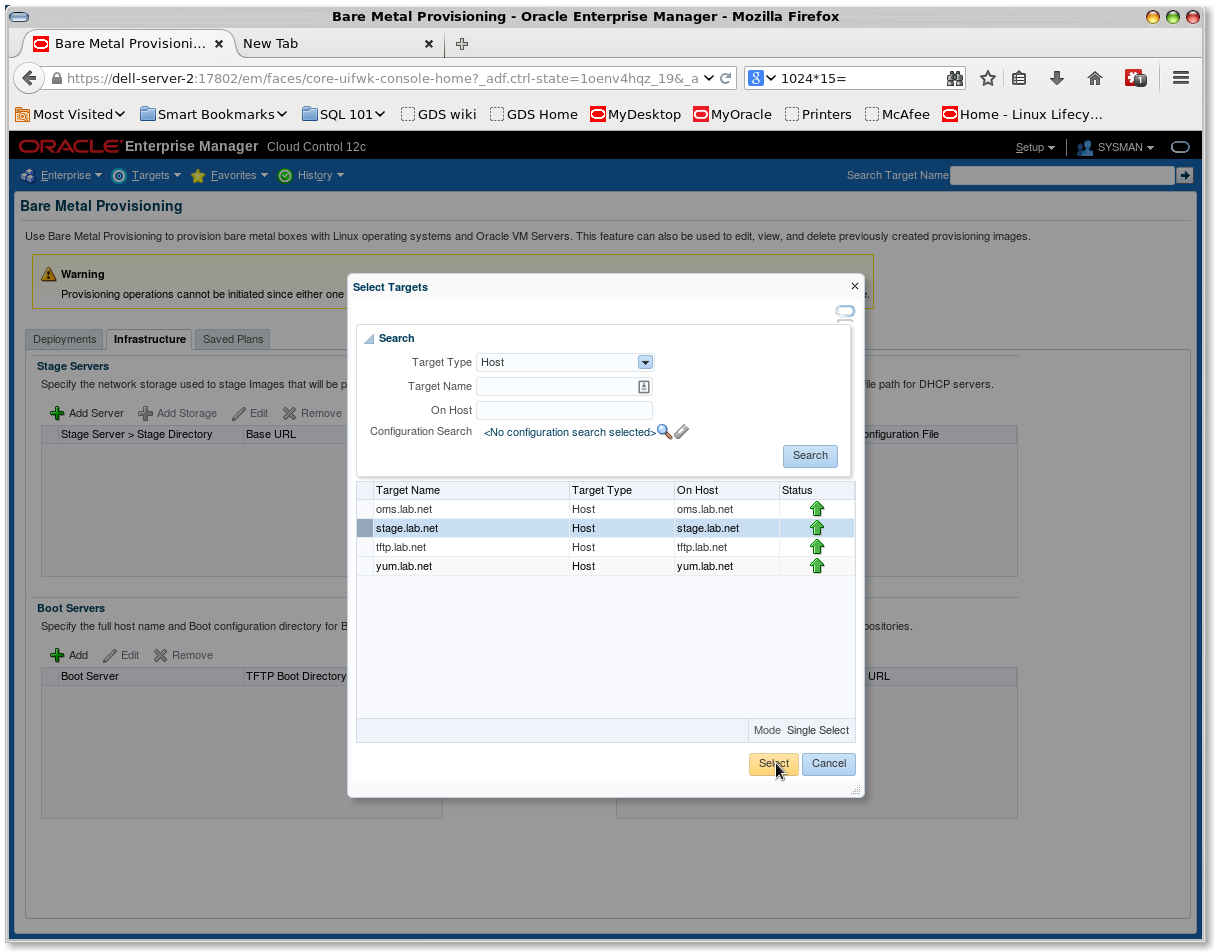
\includegraphics[width=.9\linewidth]{./images/Stage_server_selection.png}
\caption{Stage Server Selection}
\end{figure}
\clearpage

This will bring you back to the 'Add Stage Server' wizard. Add the next two propeties manually:

\begin{center}
\begin{tabular}{ll}
Property & Value\\
\hline
Stage Directory & /stage\\
Base URL & \url{file://stage.lab.net/stage}\\
\end{tabular}
\end{center}

It is very important to get these values correct. Be careful and check your work. A failure to get these values correct isn't easy to figure out later!

Add a Boot server similarly. The property values required are:

\begin{center}
\begin{tabular}{ll}
Property & Value\\
\hline
Boot server & tftp.lab.net\\
TFTP Boot Directory & /tftpboot\\
\end{tabular}
\end{center}

Again, check these values carefully!

We won't be using OEM to modify a DHCP server, so we don't configure one (its optional).

Add an RPM Repository, using the following property values:

\begin{center}
\begin{tabular}{ll}
Property & Value\\
\hline
Repository Name & OL6 Repository\\
Complete URL & \url{http://yum.lab.net/ol6}\\
\end{tabular}
\end{center}

When this process is completed the infrastructure page (with the 'Stage Server' expanded) should look like this:
\begin{figure}[htb]
\centering
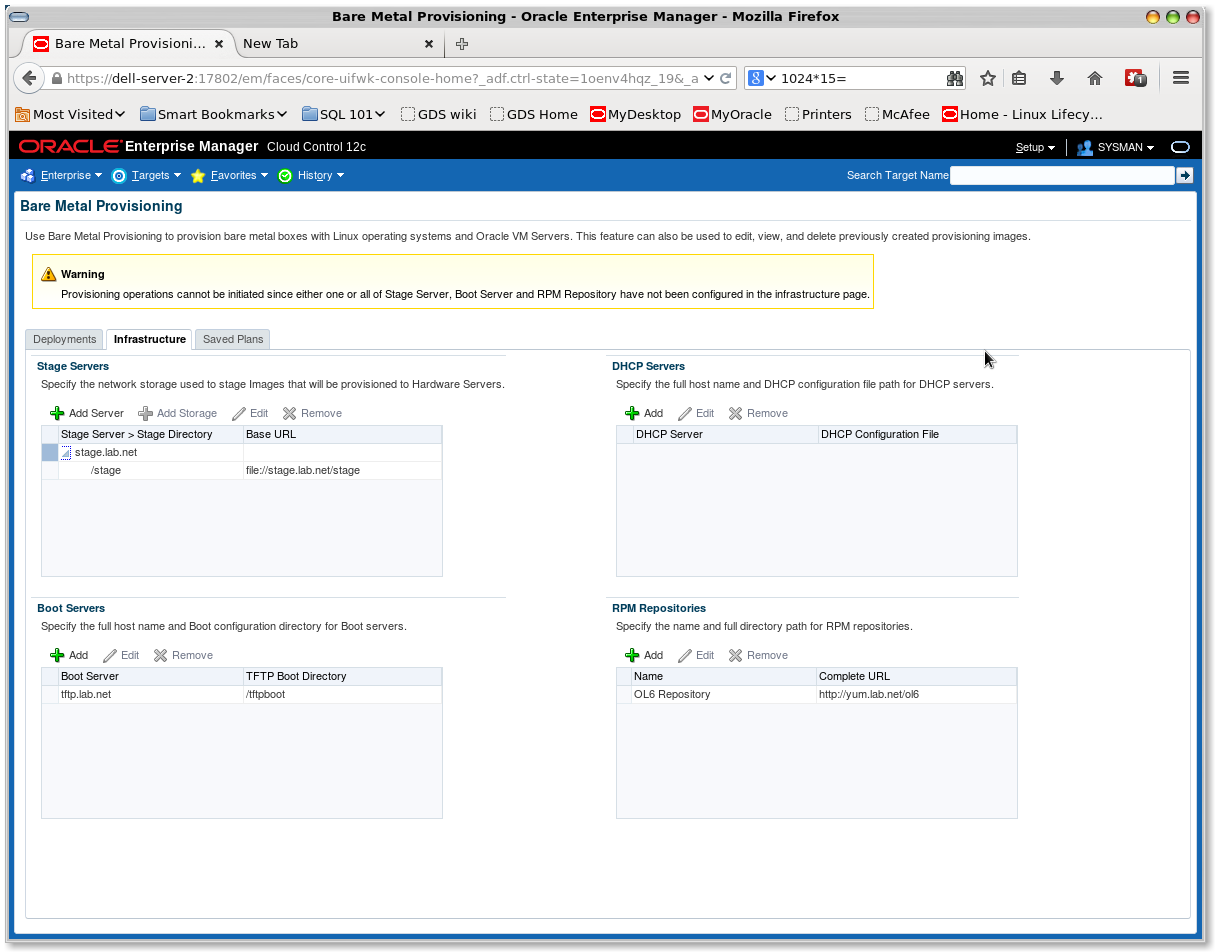
\includegraphics[width=.9\linewidth]{./images/Infra_review.png}
\caption{Infrastructure Setup Review}
\end{figure}
\clearpage

Returning to the 'Deployments' tab will finalize this setup and the previous warning will no longer be shown:
\begin{figure}[htb]
\centering
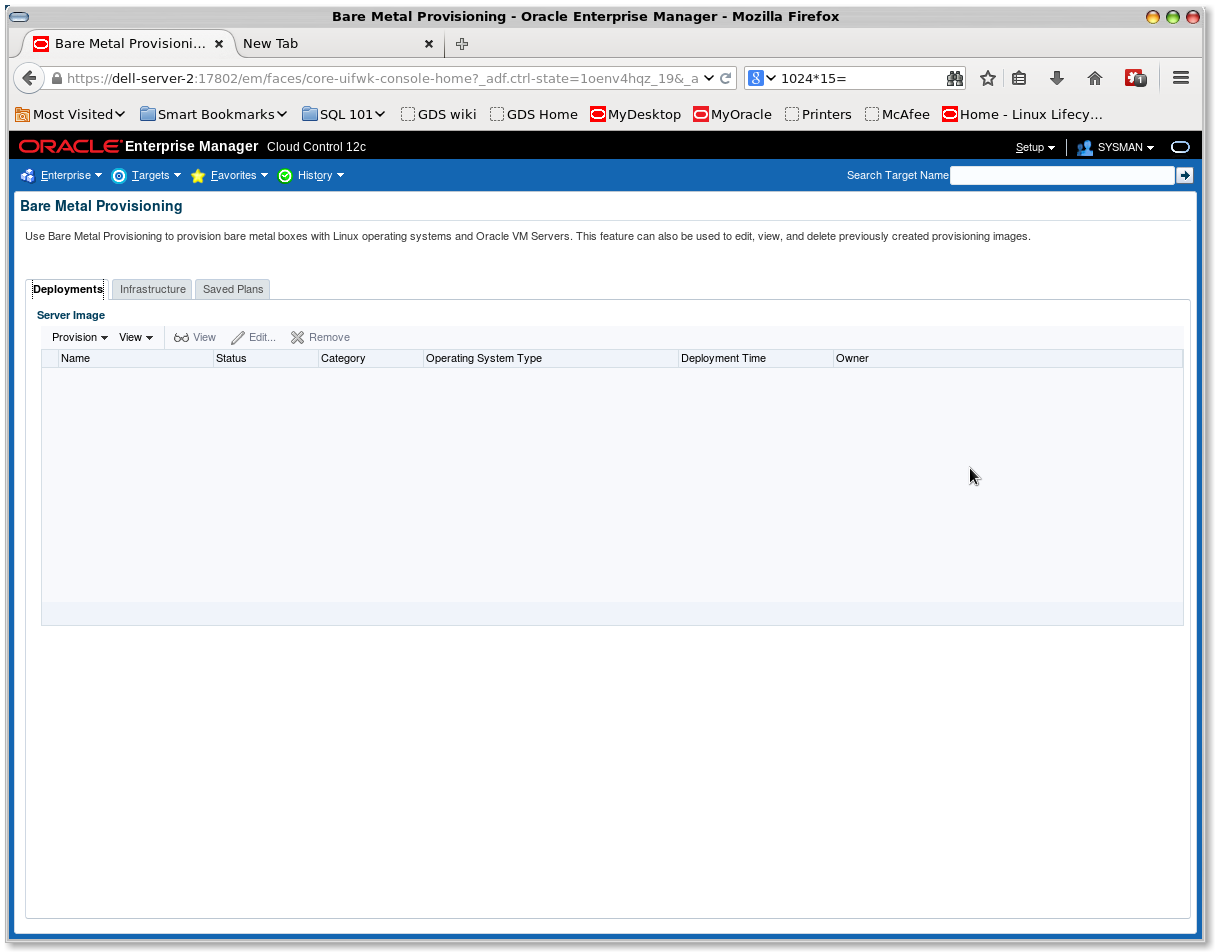
\includegraphics[width=.9\linewidth]{./images/Infra_Complete.png}
\caption{Infrastructure Setup Completed}
\end{figure}
\clearpage
\subsection{Snapshot}
\label{sec-4-5}
\section{Demo Operation}
\label{sec-5}
% Emacs 24.4.1 (Org mode 8.2.10)
\end{document}
